\documentclass[12pt]{article}
\usepackage{float}
\usepackage{harvard}
\usepackage[acronym]{glossaries}
\usepackage[automake]{glossaries-extra}
\usepackage[table,xcdraw]{xcolor}
\usepackage{pgfgantt}
\usepackage{graphicx}
\usepackage{array}
\usepackage{multirow}
\usepackage{pdflscape}
\usepackage{pdfpages}
\usepackage[hidelinks]{hyperref}
\usepackage{listings}
\usepackage{xcolor}
\usepackage[noabbrev,capitalize,nameinlink]{cleveref}
\usepackage{amssymb}
\usepackage{longtable}



\graphicspath{ {./images/} }


\makeglossaries

\newglossaryentry{ictal}
{
        name=latex,
        description={Is a mark up language specially suited for 
scientific documents}
}

\newglossaryentry{preictal}
{
        name=latex,
        description={Is a mark up language specially suited for 
scientific documents}
}

\definecolor{codegreen}{rgb}{0,0.6,0}
\definecolor{codegray}{rgb}{0.5,0.5,0.5}
\definecolor{codepurple}{rgb}{0.58,0,0.82}
\lstdefinestyle{pythonstyle}{
  language=Python,
  basicstyle=\small\ttfamily,
  commentstyle=\color{codegreen},
  keywordstyle=\color{blue},
  numberstyle=\tiny\color{codegray},
  stringstyle=\color{codepurple},
  breaklines=true,
  breakatwhitespace=true,
  numbers=left,
  numbersep=5pt,
  showstringspaces=false,
  tabsize=4,
}

\lstdefinestyle{logstyle}{
  basicstyle=\small\ttfamily,
  breaklines=true,
  breakatwhitespace=true,
  numbers=none, % No line numbers for log output
  frame=none, % No frame for log output
}

%\acrshort{gcd}
%\acrfull{gcd}
\newacronym{eeg}{EEG}{Electroencephalogram}
\newacronym{eegs}{EEGs}{Electroencephalograms}
\newacronym{ai}{AI}{Artificial Intelligence}
\newacronym{ml}{ML}{Machine Learning}
\newacronym{snr}{SNR}{Signal-to-Noise Ratio}
\newacronym{emd}{EMD}{Empirical Mode Decomposition}
\newacronym{imf}{IMF}{Intrinsic Mode Functions}
\newacronym{csp}{CSP}{Common Spatial Pattern}
\newacronym{ga}{GA}{Genetic Algorithm}
\newacronym{loocv}{LOOCV}{Leaving One Out Cross-Validation}
\newacronym{ann}{ANN}{Artificial Neural Network}
\newacronym{mlpann}{MP-ANN}{Multi-layer Perceptron Artificial Neural Network}
\newacronym{dwt}{DWT}{Discrete Wavelet Transformation}
\newacronym{rnn}{RNN}{Recurrent Neural Network (Elman)}
\newacronym{cnn}{CNN}{Convolutional Neural Network}
\newacronym{svm}{SVM}{Support Vector Machine}
\newacronym{knn}{kNN}{K Nearest Neighbor}
\newacronym{lr}{LR}{Logistical Regression}
\newacronym{pca}{PCA}{Principal Component Analysis}
\newacronym{rf}{RF}{Random Forest}
\newacronym{memd}{MEMD}{Multivariate Empirical Mode Decomposition}
\newacronym{stft}{STFT}{Short-Time Fourier Transform}
\newacronym{chb}{CHB-MIT}{Children's Hospital Boston}
\newacronym{edf}{EDF}{European Data Format}
\newacronym{dstl}{DSTL}{Dynamical Entrainment; difference of short-term Lyapunov exponents}
\newacronym{splv}{SPLV}{Phase-locking Synchrony}
\newacronym{oop}{OOP}{Object-oriented Programming}
\newacronym{csv}{CSV}{Comma-separated values}
\newacronym{oom}{OOM}{Out of Memory}

\title{Real-time preictal detection through the application of machine learning to Electroencephalogram signals.}
\author{William Riddell}
\date{\parbox{\linewidth}{\centering
\vspace{0.5cm}
\today\endgraf\bigskip\vspace{0.5cm} 
Word Count: 10,000 \\ \vspace{0.5cm}  
Supervised by Kashinath Basu}}



\begin{document}

\includepdf[pages=-]{cover.pdf}

\maketitle

\vfill 
\begin{center} 
Faculty of Technology, Design and Environment\\
School of Engineering, Computing and Mathematics
\end{center}
\pagebreak
\tableofcontents
\listoffigures
\listoftables
\printglossary[type=\acronymtype]
\pagebreak


\section{Abstract}

“Epilepsy is one of the most common serious brain conditions, affecting over 70 million people worldwide.” \cite{thijs2019epilepsy} Antiepileptic Drugs have been developed and are currently in widespread use, however, “one third of people with epilepsy will not have adequate seizure control with the current medications [available Antiepileptic Drugs (AEDs)]. For these patients, the situation has improved very little in the last few decades” \cite{galanopoulou2012identification}. Furthering this, 35\% of epilepsy patients become resistant to AED medication \cite{moghim2014predicting}. This paints a bleak situation for people suffering from epilepsy; “There is an urgent need for more effective and better-tolerated treatments'' \cite{loscher2011modern}.

This project describes a non-intrusive solution that classifies the current state of a patient in real-time. A preprocessing and classification pipeline has been developed which classifies \acrfull{eeg} signals into one of three categories (interictal, preictal, or ictal) through the use of an \acrfull{cnn} and \acrfull{stft}. This project has also tuned a selection of models, with 15 different models boasting 100\% accuracy against a validation dataset.




\section{Acknowledgements}

I would like to thank my project supervisor, Kashinath Basu for his support throughout the project. Our weekly meetings gave invaluable advice and direction which helped me stay on track and encouraged me to develop a project which I am incredibly proud of. 


\section{Introduction}


Over the last 20 years, \acrfull{ai} has seen a large evolution through the use of \acrfull{ml}; the statistical analysis of data which leads to the unveiling of characteristics and connections. \cite{awad2015efficient}. There has been a large uptake of applying \acrshort{ml} techniques to biomedical data, increasing the speed and accuracy of prediction, detection, diagnosis, and prognosis. 

\acrfull{eegs} measure the electrical signals in the brain. \acrshort{eegs} have a great use in giving an insight into the inner workings of the brain, for example allowing us to pick up abnormalities preceding and during their occurrence. ``A seizure is a burst of uncontrolled electrical activity between brain cells (also called neurons or nerve cells) that causes temporary abnormalities in muscle tone or movements (stiffness, twitching or limpness), behaviors, sensations or states of awareness.'' \cite{johnHopkinsTypesOfSeizures} Due to this, monitoring the brain's electrical activity through the use of an \acrshort{eeg}, and applying analysis through an \acrshort{ml} model may allow us to detect the preictal period. ``An automated accurate prediction of seizures will significantly improve the quality of life of patients and reduce the burden on caregivers'' \cite{acharya2018automated}


\subsection{Background}

``Because of their unpredictable nature, uncontrolled seizures represent a major personal handicap and source of worry for patients. In addition, persistent seizures constitute a considerable burden on healthcare resources.'' \cite{assi2017towards} Due to this both medication and surgery are available to applicable patients, although with ~30\% patients being refractory to drug therapy, and an equally bleak surgery success rate; ~75\% in lesional cases, and ~50\% in nonlesional cases for temporal lobe cases along with ~60\% in lesional cases and merely ~35\% in nonlesional for frontal lobe cases \cite{assi2017towards}, a large population of patients would therefore greatly benefit from a prediction system in their daily life. 

\subsection{Aim and Objectives}

This project will aim to develop a consistent \acrshort{ml} model trained to classify either preictal, interictal, and ictal periods. The model will have to achieve a high degree of accuracy ($\geq90\%$) when being applied to \acrshort{eeg} data in real time. Furthermore, a real-time simulation will need to be developed along with an \acrshort{ml} pipeline and model parameter tuning.

 
\paragraph{Objectives} \label{objectives}

\begin{enumerate}
\item Research and find a suitable dataset allowing for the classification of the interictal, preictal, and ictal periods.
\item Research and find an suitable \acrshort{ml} model approach.
\item Create a data preparation and preprocessing pipeline that extracts the dataset into an \acrshort{ml} format suitable for training and testing.
\item Undergo parameter tuning and model architecture tuning of the selected \acrshort{ml} model approach.
\item Produce a simulation interface that streams \acrshort{eeg} data in real-time through the preprocessing pipeline and into the optimal model. The simulation should show the current classification to the user every second.
\end{enumerate}

\subsection{Project Requirements}\label{requirements}

The formal requirements of this project are stated in

\begin{enumerate}
\item{Develop and preprocessing pipeline which accepts raw \acrshort{eeg} data.}
\item{Tune a number of models to find the optimal variable configuration.}
\item{Ensure that the optimal model has an accuracy of $\geq90\%$ against a validation dataset.}
\item{From \acrshort{eeg} data extraction to prediction, the process must take at most 1 second.}
\item{Create a real-time simulation mimicking a real-life application.}
\end{enumerate}

\section{Background Review}

\subsection{Datasets}\label{datasets}

\cite{wong2023eeg} reviews 10 datasets available to download. It evaluates the way the \acrshort{eegs} were physically setup on the subject, the subjects themselves, and the data's properties. Wong et al. also state their opinion on what tasks suit what dataset, with the main two tasks being either detection or prediction. 

\begin{table}[H]
\centering
\begin{tabular}{l}
\textbf{Dataset}                       \\
University of Bonn                   \\
CHB-MIT Scalp EEG                    \\
Melbourne-NeuroVista seizure trial (Neurovista Ictal)                           \\
Kaggle UPenn and Mayo Clinic's Seizure Detection Challenge                     \\
Neurology and Sleep Centre Hauz Khas \\
Kaggle American Epilepsy Society Seizure Prediction Challenge                  \\
Kaggle Melbourne-University AES-MathWorks-NIH Seizure Prediction Challenge \\
TUH EEG Seizure Corpus (TUSZ)        \\
Siena Scalp EEG                      \\
Helsinki University Hospital EEG    
\end{tabular}
\caption{The Datasets analysed}
\end{table}

Within these datasets, Wong et al. were also able to find the way the EEG nodes were positioned on the subject's cranium, along with whether the EEG nodes were either placed intracranial or extracranial. Wong et al. also the number of channels that are contained in the raw EEG data for each dataset.

\begin{table}[H]
\centering
\begin{tabular}{p{0.4\textwidth}p{0.1\textwidth}p{0.2\textwidth}p{0.2\textwidth}}
\textbf{Dataset}                                              & \textbf{Number of channels} & \textbf{Placement method}                & \textbf{Type of signal} \\
University of Bonn                                            & 1                           & International 10–20 system, Intracranial & Scalp/Intracranial EEG  \\
CHB-MIT Scalp EEG                                             & 18                          & International 10–20 system/Nomenclature  & Scalp EEG               \\
Melbourne-NeuroVista seizure trial (NeuroVista Ictal)         & 16                          & Intracranial                             & Intracranial EEG        \\
Kaggle UPenn and Mayo Clinic's Seizure Detection Challenge    & 16–76                       & Intracranial                             & Intracranial EEG        \\
Kaggle American Epilepsy Society Seizure Prediction Challenge & 16                          & Intracranial                             & Intracranial EEG        \\
Neurology and Sleep Centre Hauz Khas                          & 1                           & International 10–20 System               & Scalp EEG               \\
Kaggle Melbourne-University AES-MathWorks-NIH Seizure Prediction Challenge Data & 16 & Intracranial & Intracranial EEG \\
TUH EEG Seizure Corpus (TUSZ)                                 & 23–31                       & International 10–20 system / Nomenclature & Scalp EEG               \\
Helsinki University Hospital EEG                              & 19                          & International 10–20 system               & Scalp EEG               \\
Siena Scalp EEG                                               & 20/29                       & International 10–20 system/Nomenclature  & Scalp EEG              
\end{tabular}
\caption{Channel Characteristics}
\end{table}

Wong et al. also noted along with this data that the ``University of Bonn dataset contains a mixture of both scalp and intracranial EEG data where scalp EEG from healthy subjects was taken, while intracranial EEG was taken from subjects with a history of seizures.'' \cite{wong2023eeg}. This may present a skew on the \acrshort{ml} model during training.


\begin{table}[H]
\centering
\begin{tabular}{p{0.4\textwidth}p{0.2\textwidth}p{0.2\textwidth}p{0.2\textwidth}}
  \textbf{Dataset} &
  \textbf{Noncontinuous data} &
  \textbf{Short-term continuous data} &
  \textbf{Continuous data} \\
  
University of Bonn                                                              & Yes & No  & No  \\
CHB-MIT Scalp EEG                                                               & No  & Yes & Yes \\
Melbourne-NeuroVista seizure trial (Neurovista Ictal)                           & N/A & N/A & N/A \\
Kaggle UPenn and Mayo Clinic's Seizure Detection Challenge                      & Yes & No  & No  \\
Kaggle American Epilepsy Society Seizure Prediction Challenge                   & Yes & No  & No  \\
Neurology and Sleep Centre Hauz Khas                                            & Yes & No  & No  \\
Kaggle Melbourne-University AES-MathWorks-NIH Seizure Prediction Challenge Data & Yes & No  & No  \\
TUH EEG Seizure Corpus (TUSZ)                                                   & No  & Yes & No  \\
Helsinki University Hospital EEG                                                & No  & Yes & No  \\
Siena Scalp EEG                                                                 & No  & Yes & No 
\end{tabular}
\caption{Temporal properties}
\end{table}

Wong et al. ordered the datasets into groups, either continuous or noncontinuous data. For the continuous data they separated out datasets that record for less than 24 hours in a single go, these were classified as ``Short-term continuous'' data.

\begin{table}[H]
\centering
\begin{tabular}{p{0.4\textwidth}p{0.2\textwidth}p{0.2\textwidth}p{0.2\textwidth}}
\textbf{Dataset}                                                                & \textbf{Number of subjects} & \textbf{Subject type} & \textbf{} \\
University of Bonn                   & 10  & Human &  \\
CHB-MIT Scalp EEG                    & 23  & Human &  \\
Melbourne-NeuroVista seizure trial (NeuroVista Ictal)                           & 12                          & Human                 &           \\
Kaggle UPenn and Mayo Clinic's Seizure Detection Challenge                      & 12                          & Human \& Canine       &           \\
Kaggle American Epilepsy Society Seizure Prediction Challenge                   & 7                           & Human \& Canine       &           \\
Neurology and Sleep Centre Hauz Khas & 10  & Human &  \\
Kaggle Melbourne-University AES-MathWorks-NIH Seizure Prediction Challenge Data & 3                           & Human                 &           \\
TUH EEG Seizure Corpus (TUSZ)        & 642 & Human &  \\
Helsinki University Hospital EEG     & 79  & Human &  \\
Siena Scalp EEG                      & 14  & Human & 
\end{tabular}
\caption{Subject properties}
\end{table}

Wong et al. also were able to identify the number of subjects within each dataset. Within the two ``Kaggle'' datasets there are Canine subjects, making them unsuitable for this project. 

Within the review, they also produced tables displaying the segment information for each dataset, breaking down the recording length and frequency, along with the number of events and segments. This information should not weigh into which dataset suits the idea of preictal prediction so shall be left out in this background review. Wong et al. also discussed the idea of the class imbalance problem, where the number and length of each ictal period are unbalanced. Two datasets, ``University of Bonn'' and the ``Neurology and Sleep Centre Hauz Khas'' have addressed this issue and have balanced their data between ictal, preictal, interictal, and neonatal periods.

Taking the research into account Wong et al. suggested which dataset suits either prediction or detection. ``Since the aim of seizure prediction is to forecast impending seizures, EEG recordings that include preictal and interictal data should be used for the study, while the aim of seizure detection is to detect ongoing seizure events, hence, EEG recordings that contain ictal and interictal data should be used.'' \cite{wong2023eeg}.

\begin{table}[H]
\centering
\begin{tabular}{p{0.5\textwidth}p{0.4\textwidth}}
\textbf{Dataset}                     & \textbf{Application}         \\
University of Bonn                   & Seizure detection            \\
CHB-MIT Scalp EEG                    & Seizure detection/Prediction \\
Melbourne-NeuroVista seizure trial (NeuroVista Ictal)                           & Seizure detection/Prediction \\
Kaggle UPenn and Mayo Clinic's Seizure Detection Challenge                      & Seizure detection            \\
Kaggle American Epilepsy Society Seizure Prediction Challenge                   & Seizure prediction           \\
Neurology and Sleep Centre Hauz Khas & Seizure detection/Prediction \\
Kaggle Melbourne-University AES-MathWorks-NIH Seizure Prediction Challenge Data & Seizure prediction           \\
TUH EEG Seizure Corpus (TUSZ)        & Seizure detection/Prediction \\
Helsinki University Hospital EEG     & Seizure detection/Prediction \\
Siena Scalp EEG                      & Seizure detection/Predictio 
\end{tabular}
\caption{Suggested applications}
\label{dataset_applications}
\end{table} 

\subsection{\acrfull{ml} Models}\label{models}

A series of papers have been reviewed with the following \acrshort{ml} model types and feature extraction processes being used:

\begin{itemize}
	\item \acrfull{ml} models
	\begin{itemize}
	\item \acrfull{knn}.
	\item \acrfull{svm}.
	\item \acrfull{lr}.
	\item \acrfull{cnn}.
	\end{itemize}
	\item Preprocessing Pipelines
	\begin{itemize}
	\item Time domain, using the third order Butterworth bandpass filter.
	\item Frequency domain using the Fourier transform.
	\item Time-Frequency domain using Wavelet Decomposition.
	\item Cross-correlation.
	\item Non-linear Interdependence.
	\item \acrfull{dstl}.
	\item \acrfull{splv}.
	\item Entropy of the phase difference.
	\item Wavelet Coherence.
	\item \acrfull{stft}
	\end{itemize}
\end{itemize}

\paragraph{\acrfull{knn} and \acrfull{svm}}\mbox{}\\

\cite{savadkoohi2020machine} built a feature extraction process that extracted the ``time domain" using the Butterworth filter (1-70 Hz) \ref{eq:butterworth}, the ``frequency domain" using a Fourier transform  \ref{eq:fourier}, and the ``time-frequency domain" using Wavelet decomposition for the entire dataset. The resulting data is then split into its 5 brain wave bands; Delta, Theta, Alpha, Beta, and Gamma. From these 4 variables were extracted, mean, variance, skewness, and kurtosis, leading to 60 total extracted features. 

\begin{figure}[H]
\[ y(n) = \sum_{i=0}^{N} a_i \cdot x(n - i) + \sum_{j=1}^{N} b_j \cdot y(n - j) \]
\caption{Third Order Butterworth bandpass filter}
\label{eq:butterworth}
\end{figure}

\begin{figure}[H]
\[ \widehat{f}(\xi) = \int_{-\infty}^{\infty} f(x)\ e^{-i 2\pi \xi x}\,dx. \]
\caption{Fourier transform equation}
\label{eq:fourier}
\end{figure}

A prediction was calculated from an \acrshort{knn} and \acrshort{svm} model for each separate domain. The results are shown in \ref{tab:svm_knn} showing the potential of each model.

\begin{table}[H]
\centering
\begin{tabular}{llll}
\multirow{2}{*}{Model}         & \multicolumn{3}{l}{Accuracy \%} \\
                               & TD & FD & T-FD\\
\protect\acrfull{svm} & 99.5        & 100              & 100                   \\
\protect\acrfull{knn} & 99.5        & 99               & 99.5                 
\end{tabular}
\caption{Results from \protect\cite{savadkoohi2020machine} showing results for the Time Domain, Frequency Domain, and Time-Frequency Domain}
\label{tab:svm_knn}
\end{table}

The classification times however were not included in the report. Extraction in real-time may not be applicable for an approach so extensive in its feature extraction. 

\paragraph{\acrfull{lr}, \acrfull{svm}, and \acrfull{cnn}}\mbox{}\\

Mirowski et al. used the \cite{freiburg_eeg} dataset containing intracranial recordings and measured the performance of an \acrshort{lr}, \acrshort{svm}, and \acrshort{cnn} \acrshort{ml} models. They compiled 6 different preprocessing pipelines and tested the selected models against each. The preprocessing pipelines are as follows: 

\begin{itemize}
\item The Cross-correlation between pairs of EEG channels was calculated with delays ranging from -0.5 to 0.5. The delays allowed for the propagation and processing time of brainwaves. Cross-correlation describes the amount $f$ has to be shifted along the $x$ axis to equal $g$\ref{eq:crossCorrelation}. Only the maximum value of the cross-correlation values was retained for training.

\begin{figure}[H]
\[ (f \star g)(\tau)\ \triangleq \int_{-\infty}^{\infty} \overline{f(t)} g(t+\tau)\,dt \]
\caption{Cross-Correlation}
\label{eq:crossCorrelation}
\end{figure}

\item Non-linear interdependence ``which measures the distance, in state-space, between time-delay embedded trajectories of two EEG channels'' was also extracted. This is a bivariate feature that ``measures the Euclidian distance, in reconstructed state-space, between trajectories described by two EEG channels''.

\item The third method was \acrfull{dstl}, where a Lyapunov exponent \ref{eq:lyapunov} describes the rate of separation for two trajectories, which in this report was based off ``a common measure of the chaotic nature of a signal'' \cite{mirowski2009classification}

\begin{figure}[H]
\[ \lambda = \lim_{t \to \infty} \lim_{|\delta \mathbf{Z}_0| \to 0} \frac{1}{t} \ln\frac{| \delta\mathbf{Z}(t)|}{|\delta \mathbf{Z}_0|} \]
\caption{Maximal Lyapunov ($\lambda$) exponent}
\label{eq:lyapunov}
\end{figure}

\item The last 3 features were \acrfull{splv}, Entropy, and Coherence of the phase difference. These were extracted from the wavelet transformation The wavelet transformation extracts the frequency-specific and time-dependent phases.

\begin{figure}[H]
\[ SPLV_{a,b}(f) = \frac{1}{N} \sum_{l=1}^{N} e^{i\left(\phi_{a,f}(l) - \phi_{b,f}(l)\right)} \]
\caption{\acrfull{splv} extraction from the wavelet transformation}
\label{eq:splv}
\end{figure}

\end{itemize}

The following results show the number of patients with perfect seizure prediction results ``(no false positives, all seizures predicted)'' from \cite{mirowski2009classification} for each model, for each preprocessing pipeline.

\begin{table}[H]
\centering
\begin{tabular}{lll}
\multicolumn{3}{l}{Cross-Correlation} \\
\acrshort{lr}          & \acrshort{cnn}        & \acrshort{svm}        \\
4           & 9          & 4          \\
19\%        & 43\%       & 19\%      
\end{tabular}
\caption{Cross-Correlation results.}
\end{table}

\begin{table}[H]
\centering
\begin{tabular}{lll}
\multicolumn{3}{l}{Non-Linear interdependence} \\
\acrshort{lr}          & \acrshort{cnn}        & \acrshort{svm}        \\
3              & 10            & 5             \\
19\%           & 48\%          & 24\%         
\end{tabular}
\caption{Non-Linear interdependence results.}
\end{table}

\begin{table}[H]
\centering
\begin{tabular}{l}
\acrshort{dstl} \\
\acrshort{svm}  \\
1    \\
5\% 
\end{tabular}
\caption{\acrfull{dstl} results.}
\end{table}


\begin{table}[H]
\centering
\begin{tabular}{lll}
\multicolumn{3}{l}{\acrshort{splv}} \\
\acrshort{lr}          & \acrshort{cnn}        & \acrshort{svm}        \\
10     & 13     & 7      \\
48\%   & 62\%   & 33\%  
\end{tabular}
\caption{\acrfull{splv} results.}
\end{table}

\begin{table}[H]
\centering
\begin{tabular}{lll}
\multicolumn{3}{l}{Entropy of Phase Difference} \\
\acrshort{lr}          & \acrshort{cnn}        & \acrshort{svm}        \\
9              & 11             & 7             \\
43\%           & 52\%           & 33\%         
\end{tabular}
\caption{Entropy of Phase Difference results. }
\end{table}

\begin{table}[H]
\centering
\begin{tabular}{lll}
\multicolumn{3}{l}{Distribution of Wavelet Coherence} \\
\acrshort{lr}          & \acrshort{cnn}        & \acrshort{svm}        \\
11               & 15               & 8               \\
52\%             & 71\%             & 38\%           
\end{tabular}
\caption{Distribution of Wavelet Coherence results.}
\end{table}


These results show the strength of an \acrshort{cnn} when compared to other \acrshort{ml} models as it's obtained the highest results across all tables. \acrshort{lr} however can also achieve strong results when paired with the correct preprocessing pipeline. Both methods would be applicable for this project assuming that the time from recording to final prediction is less than a second.

\paragraph{\acrfull{cnn}}\mbox{}\\

Another \acrshort{cnn} approach was implemented by Truong et al. \cite{truong2018convolutional} who applied an \acrfull{stft} transform \ref{eq:stft} on 30 seconds of \acrshort{eeg} data. Interference was then removed from the produced matrices by applying a notch filter. The final result was then fed into an \acrshort{cnn} producing these results:

\begin{table}[H]
\centering
\begin{tabular}{lll}
No. of seizures & Sensitivity (\%) & False Positive Rate (/h) \\
59              & $81.4 \pm 0.0$   & $0.06 \pm 0.00$         
\end{tabular}
\caption{Cross-Correlation results. }
\label{tab:my-table}
\end{table}


\section{Project Methodology and Development}\label{development}

\subsection{Methodology}

\subsubsection{Approach}

From the datasets discussed in \ref{datasets}, the \acrfull{chb} \acrshort{eeg} dataset has been chosen due to the large amount of continuous data, suitable for extracting the preictal period \ref{dataset_applications}. The dataset also has \acrshort{eeg} nodes positioned on the subject's scalps, fitting with the use case of this project. Furthermore, the \acrshort{chb} \acrshort{eeg} dataset has produced summary plain-text files for each of the subject's recordings, stating when every seizure began and ended allowing for a straightforward methodology when configuring the \acrshort{eeg} tuning and training environment.

Through the analysis of various \acrshort{ml} models an \acrshort{cnn} will be used for this project. Both \cite{truong2018convolutional} and \cite{mirowski2009classification} show the potential \acrshort{cnn} have when being used in preictal prediction. The approach described in \cite{truong2018convolutional} was able to achieve similar or better results in comparison with other preprocessing pipelines and/or \acrshort{ml} model configurations while using a less computationally intense preprocessing method. This method was based around an \acrshort{stft} extraction and is described in \cite{truong2018convolutional}. This may allow for the classification to be done in real-time, meeting the project's objectives \ref{objectives}. To ensure this requirement is met a real-time simulation will be developed, showing the raw EEG data and the final prediction every second.
%more detailed information about the cnn is discussed in section \paragraph{\acrfull{cnn}}\mbox{}\\



\subsubsection{Development System}

Due to the linear nature of this project, a Waterfall methodology will be used. Waterfall ensures that previous stages of the software are complete before moving on, this will keep the project on track and moving in a forward direction, crucial for the time-limited aspect of this project. Furthermore, due to the analysis undergone through literature reviews the direction and therefore the goals of the project are clearly defined; this further supports the choice of a Waterfall approach.

\subsubsection{Version Control}

This project will be under version control through the use of Git, along with GitHub as a remote repository. Both the dataset and the trained models will not be under version control. The use of a version control system and remote repository ensures that if anything goes awry a backup of all commits is stored remotely, securing any progress made in the project. Git also gives the benefit of many features; notably branches and stashing, allowing for developing ideas, features, and bugs without affecting the ``main'' code, and merging allows for the combination of said branches.

\subsubsection{Software and Libraries Used}

\begin{table}[H]
\centering
\begin{tabular}{p{0.3\textwidth}p{0.7\textwidth}}
Name:              & Use case:                                                                                                                               \\
Google Cloud       & Used to download the \acrshort{chb} \acrshort{eeg} dataset                                                                            \\
Keras (TensorFlow) & Used to build, train and test the \acrshort{ml} models.                                                                \\
Matplotlib         & Used in the real-time simulation to plot the Spectrogram and \acrshort{chb} \acrshort{eeg} data.                                       \\
MNE                & Provides classes for loading \acrshort{eeg} data from both CSV and \acrshort{edf} files. Also used for running an \acrfull{stft} extraction. \\
NumPy              & Utilized functions and classes to store and manipulate loaded data.                                                                     \\
Pandas             & Utilized functions and classes to store and manipulate loaded data.                                                                     \\
scikit-learn       & Provides functions used to produce performance metrics for trained \acrshort{ml} models.                       \\
nicegui.py		& An framework which allows for web-application development.       
\end{tabular}
\caption{List of Libraries used}
\label{tab:libraries}
\end{table}


\subsubsection{Schedule}\label{schedule}

The schedule describes the way the Waterfall methodology has affected the project; it shows how it's been broken down into smaller, distinct stages with progress being blocked until the previous stage has been completed. The overlap in March and April is when the models are being tuned, therefore the only active development is on the real-time simulation. 

\begin{figure}[H]
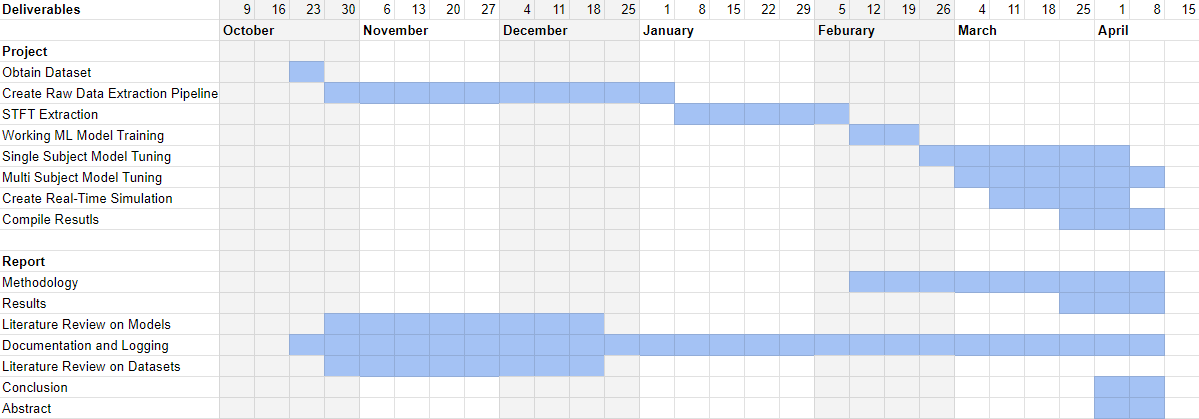
\includegraphics[width=\textwidth]{gantt}
\centering
\caption{Gantt Chart}
\label{fig:gantt}
\end{figure}




\subsection{Development}


\subsubsection{\acrfull{eeg} Data Extraction}
%include diagram for output

The \acrfull{edf} \cite{kemp1992simple} is a file format that was designed for the archival and exchange of \acrshort{eeg} recordings \cite{kemp2013european} and was the format of the \acrshort{chb} \acrshort{eeg} dataset. \acrshort{edf} files contain raw \acrshort{eeg} signals plotted against a time axis and contain metadata such as the name and recording frequency for each node. \ref{fig:eegPlot} shows an plot of raw \acrshort{eeg} data.

\begin{figure}[H]
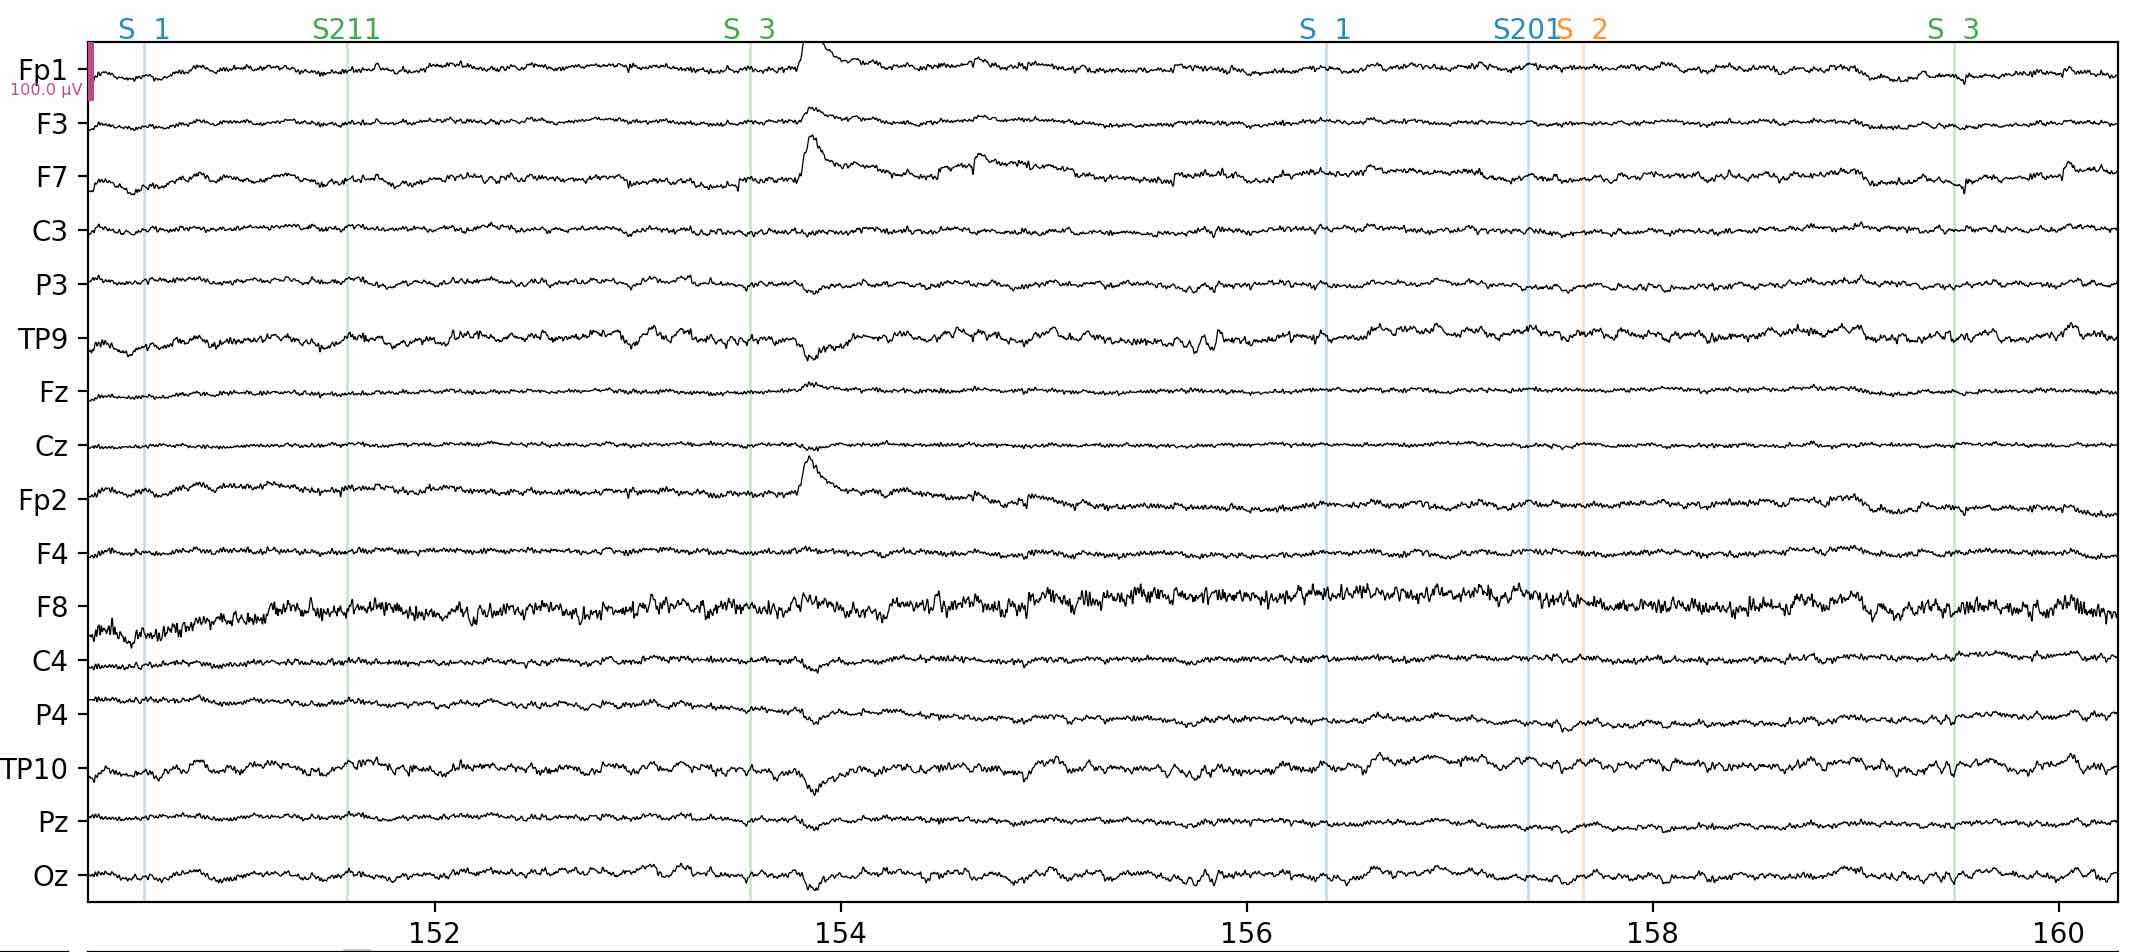
\includegraphics[width=0.8\textwidth]{eeg_raw_continuous}
\centering
\caption{Extracted raw \acrshort{eeg} data. \protect\cite{neuraldatascience2024}}
\label{fig:eegPlot}
\end{figure}

Each node's name describes its position within the internationally accepted 10-20 system shown in \ref{fig:10-20}. The 10-20 system was popularized due to its ability to cover all brain regions in a method proportional to the skull size and shape. This ensures that the inter-electrode spacing is equal, allowing for consistent measurements to be taken regardless of subject. \cite{morley201610}



\begin{figure}[H]
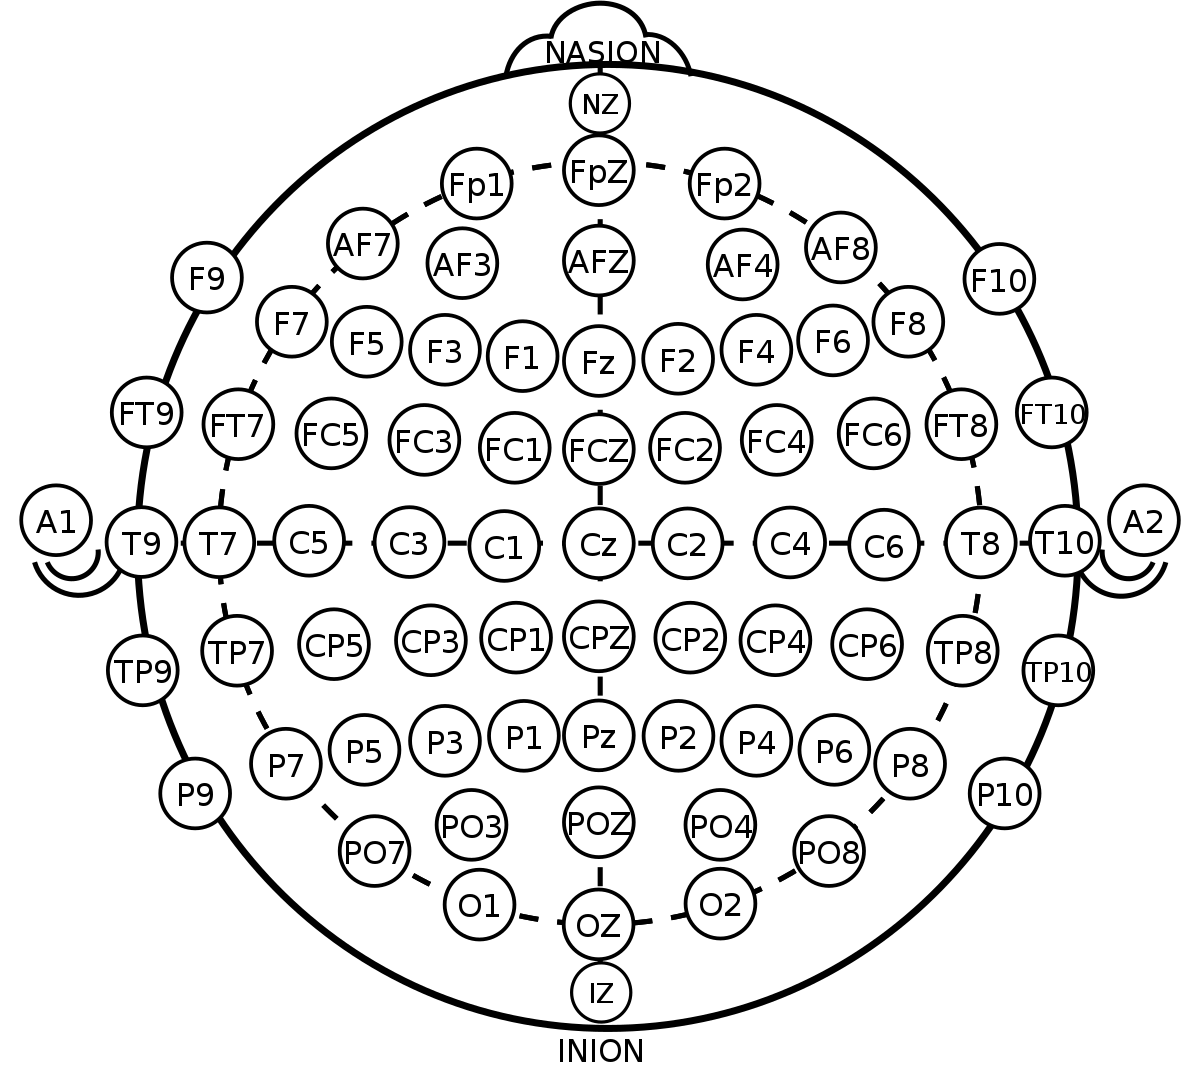
\includegraphics[width=0.6\textwidth]{10-20}
\centering
\caption{Diagram of the 10-20 International System. \protect\cite{tomaton1242010}}
\label{fig:10-20}
\end{figure}


The \acrshort{chb} dataset also contained summary files (see \ref{lst:summary-file}). From these summary files an \acrfull{oop} representation of the dataset was created. This \acrshort{oop} representation was generated for every recording and shows which subject it belonged to, the name of each \acrshort{eeg} node within the recording, also representing each node's position in the 10-20 system, the recording frequency of the \acrshort{eeg}, and any seizure's start and end times contained within that recording. This \acrshort{oop} representation allowed for the labeling of the ictal, preictal, and interictal periods.

For this project, the \acrshort{eeg} signals were extracted and stored in an \acrshort{csv} file. This allowed for a more flexible configuration of tuning scenarios such as \acrshort{eeg} node combinations or subject-specific tuning, further discussed in \ref{advancements}. Within the \acrshort{chb} \acrshort{eeg} dataset each \acrshort{eeg} configuration was not equal as some recordings contained nodes not present in other recordings. Due to this, the common channels were extracted to allow for a fair comparison of the results. There were 17 channels with the names: FP1-F7, F7-T7,T7-P7, P7-O1, FP1-F3, F3-C3, C3-P3, P3-O1, FP2-F4, F4-C4, C4-P4, P4-O2, FP2-F8, F8-T8, P8-O2, FZ-CZ, CZ-PZ. An example of the extracted data can be seen at \ref{fig:rawData}. For each recording 3 \acrshort{csv} files were created, ``/ictal/master.csv'', ``/preictal/master.csv'' and ``/interictal/master.csv''. If a period appeared more than once in a single recording it was concatenated to its corresponding ``master.csv'' file.


\begin{figure}[H]
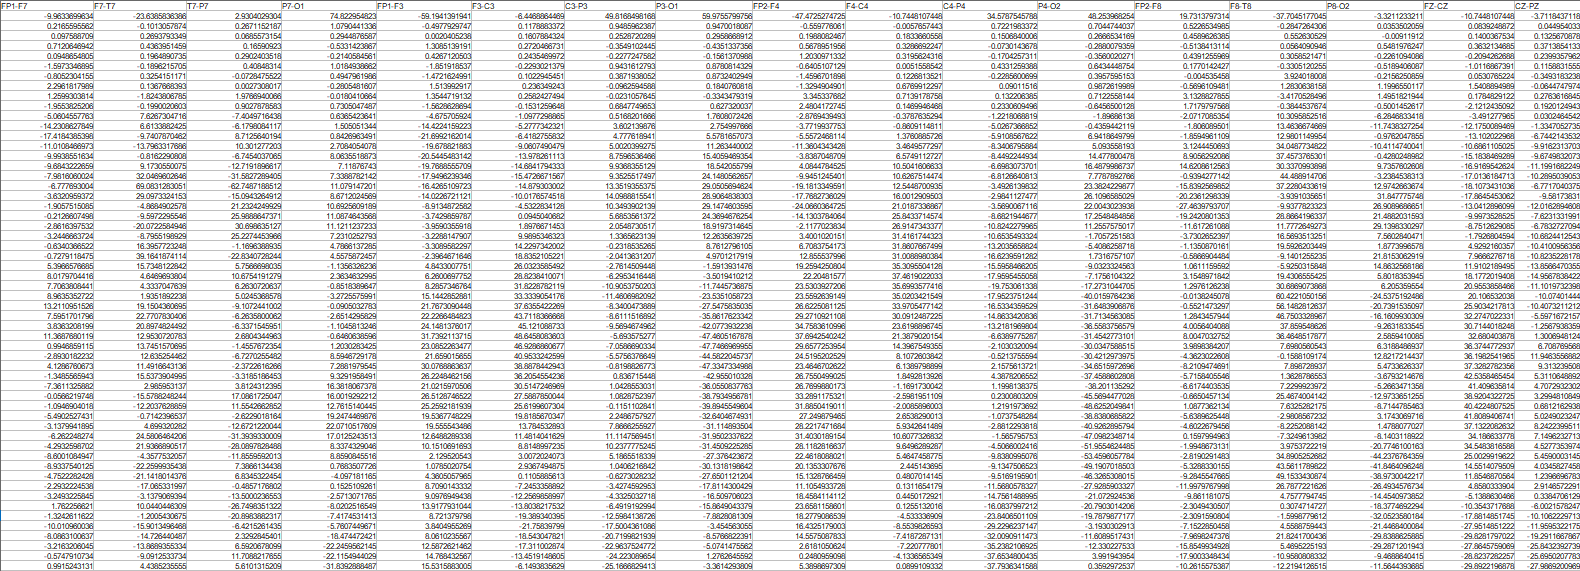
\includegraphics[width=\textwidth]{rawData}
\centering
\caption{Head of extracted \acrshort{eeg} data in \acrshort{csv} format. The shown data is approx $1/5$ second and each column represents an single \acrshort{eeg} node's data.}
\label{fig:rawData}
\end{figure}


\subsubsection{\acrfull{stft}}

\acrshort{stft} extraction is applied against \acrshort{stft} is applied to the data collected from the \acrshort{eegs} to produce an spectrogram of length 30 seconds. These images contain only a single class and were the input into the \acrshort{cnn}. \acrshort{stft} can be expressed mathematically;\\

\begin{figure}[H]
\[  \mathbf{STFT}\{x(t)\}(\tau,\omega) \equiv X(\tau, \omega) = \int_{-\infty}^{\infty} x(t) w(t-\tau) e^{-i \omega t} \, d t   \]
\caption{\acrfull{stft} Window Extraction}
\label{eq:stft}
\end{figure}

Where $w(\tau)$ is an window function and $x(t)$ is the input signal from the \acrshort{eegs}.\\


This can also be explained as taking a Fourier transform of the \acrshort{eeg} signals after a window function has been applied, and then sliding a window across the result. The sliding window transforms the one-dimensional output from the Fourier transform into two-dimensional data allowing for visual analysis.


There are various parameters for an \acrshort{stft} transformation: 
\begin{table}[H]
\centering
\begin{tabular}{p{0.3\textwidth}p{0.7\textwidth}}
Window Function & Used to isolate signal currently undergoing analysis. Optimal functions have low to no artefacts left in the signal and creates no discontinuities at section boundaries.\\
Window Size & Changes the size of the window function. This affects the resolution of both time and frequency, leading to the uncertainty principal; either variable will be in high resolution. See \ref{fig:stft1} and \ref{fig:stft2} \\
Time Step (step size or hop size) & This is the distance between windows. Influences window over or underlap, as well as directly affecting computational load. \\                            
\end{tabular}
\caption{List of \acrfull{stft} parameters}
\label{tab:stft_params}
\end{table}

For this project these variables were selected:

\begin{table}[H]
\centering
\begin{tabular}{p{0.3\textwidth}p{0.7\textwidth}}
Window Function & Sine Window: $ w[n] = \sin\left(\frac{\pi n}{N}\right) = \cos\left(\frac{\pi n}{N} - \frac{\pi}{2}\right),\quad 0\le n \le N.$ \\
Window Size & 7680. The length of the input data. \\
Time Step (step size or hop size) & 3840. This leads to an window overlap. \\                            
\end{tabular}
\caption{List of \acrfull{stft} parameters choices}
\label{tab:stft_choices}
\end{table}

See \ref{fig:stft2} for an Spectrogram produced with these parameters. 

\subsubsection{Notch Filter}

``Power line interference may severely corrupt neural recordings at 50/60 Hz and harmonic frequencies. The interference is usually non-stationary and can vary in frequency, amplitude, and phase.'' \cite{keshtkaran2014fast} This poses a large issue when training an \acrshort{ml} model against \acrshort{eeg} recordings as the interference may affect the model's ability to pick up on characteristics, or may mislead the model.

\begin{figure}[H]
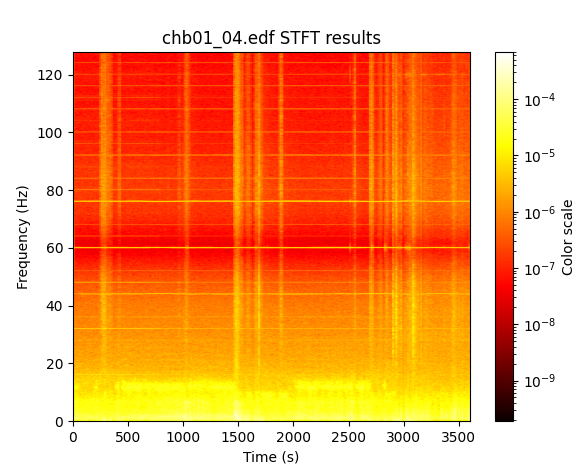
\includegraphics[width=\textwidth]{stft1}
\centering
\caption{An STFT window with high frequency resolution.}
\label{fig:stft1}
\end{figure}

\ref{fig:stft1} clearly shows power line interference with a horizontal band around 60 Hz. \cite{keshtkaran2014fast} discusses the different methods for removing power line interference, although due to the objectives stated in \ref{objectives}, a compute-intensive method needed to be avoided to allow the project to meet the real-time requirement. Through analysis done by Keshtkaran et al., a notch filter is fairly computationally light, although it does however have drawbacks such as not entirely removing the interference \cite{keshtkaran2014fast}. A notch filter was therefore applied to the raw data during the application of the \acrshort{stft} function.


\subsubsection{Synthesize Data}\label{synthesize-data}

Within the \acrshort{chb} dataset there was a class imbalance with the interictal period dwarfing all other classes for every subject. A visualization of the data can be seen bellow in \ref{tab:class-size} which was generated from the extracted data. All subjects have very little data for the preictal and ictal classes, with most of them having under 30 seconds of recorded data. If a model was trained off synthesized data for these subjects, regardless of the synthesization method, the results would be greatly misleading and the models would not work in a real-life application. Therefore it was decided that only subjects ``chb06'' and ``chb12'' will be utilized for the training and tuning of \acrshort{ml} models within this project.


\begin{table}[H]
\centering
\begin{center}
\begin{tabular}{l|lll|lll|lll}
      & \multicolumn{3}{l|}{Recordings} & \multicolumn{3}{l|}{Line Count} & \multicolumn{3}{l}{Length (Seconds)} \\
      & Ictal     & Pre     & Inter     & Ictal   & Pre     & Inter       & Ictal     & Pre       & Inter        \\ 
chb01 & 7         & 7       & 42        & 456     & 9334    & 37352484    & 1.78      & 36.46     & 145908.14    \\
chb02 & 3         & 3       & 36        & 15      & 3118    & 32489237    & 0.059     & 12.18     & 126911.08    \\
chb03 & 7         & 7       & 38        & 416     & 8201    & 35004081    & 1.625     & 32.04     & 136734.69    \\
chb04 & 3         & 3       & 42        & 2385    & 15164   & 143801293   & 9.32      & 59.23     & 561723.8     \\
chb05 & 5         & 5       & 39        & 568     & 7344    & 35927152    & 2.22      & 28.69     & 140340.44    \\
chb06 & 7         & 7       & 18        & 17803   & 41291   & 61439324    & 69.54     & 161.3     & 239997.36    \\
chb07 & 3         & 3       & 19        & 331     & 21128   & 61769049    & 1.29      & 82.53     & 241285.35    \\
chb08 & 5         & 5       & 20        & 929     & 11739   & 18420150    & 3.63      & 45.86     & 71953.71     \\
chb09 & 3         & 3       & 19        & 6648    & 19716   & 62519544    & 25.19     & 77.02     & 244216.97    \\
chb10 & 7         & 7       & 25        & 461     & 26621   & 46068086    & 1.8       & 103.99    & 179953.46    \\
chb11 & 3         & 3       & 35        & 812     & 3682    & 32052414    & 3.17      & 14.38     & 125204.74    \\
chb12 & 10        & 10      & 21        & 8058    & 10643   & 18532198    & 31.48     & 41.57     & 72391.40     \\
chb13 & 8         & 8       & 33        & 4435    & 8988    & 30391012    & 17.32     & 35.11     & 118714.90    \\
chb14 & 7         & 7       & 26        & 1608    & 12433   & 23940969    & 6.28      & 48.57     & 93519.41     \\
chb15 & 14        & 14      & 40        & 7160    & 12350   & 36843574    & 27.97     & 48.24     & 143920.21    \\
chb16 & 6         & 6       & 19        & 4381    & 5832    & 17495378    & 17.11     & 22.78     & 68341.3      \\
chb17 & 3         & 3       & 21        & 299     & 7678    & 1934639     & 1.17      & 29.99     & 75572.03     \\
chb18 & 6         & 6       & 36        & 329     & 9142    & 32822357    & 1.29      & 35.71     & 128212.33    \\
chb19 & 3         & 3       & 30        & 242     & 5657    & 27569463    & 0.95      & 22.1      & 107693.21    \\
chb20 & 6         & 6       & 29        & 2569    & 6147    & 25421628    & 10.04     & 24.01     & 99303.23     \\
chb21 & 4         & 4       & 33        & 207     & 7451    & 30240352    & 0.81      & 29.11     & 118126.34    \\
chb22 & 3         & 3       & 31        & 210     & 7004    & 28557334    & 0.82      & 27.36     & 111552.09    \\
chb23 & 3         & 3       & 9         & 12020   & 6111    & 24455749    & 46.95     & 23.87     & 95530.27    
\end{tabular}
\caption{Recording information for each subject. Valid represents if an subject has enough data, and is therefore suitable for training.}
\label{tab:class-size}
\end{center}
\end{table}


A sliding window method was used to synthesize the data for subjects ``chb06'' and ``chb12''. The sliding window method moves a window of 30s across the data at speed $x$. Variable speed allows for the generation of a specific number of windows, see \ref{fig:slidingWindow} for a diagram of this process. \ref{eq:window-size}, \ref{eq:step}, and \ref{eq:windows} were taken from the project's implementation and describe the algorithm used to synthesize the data.

\begin{figure}[H]
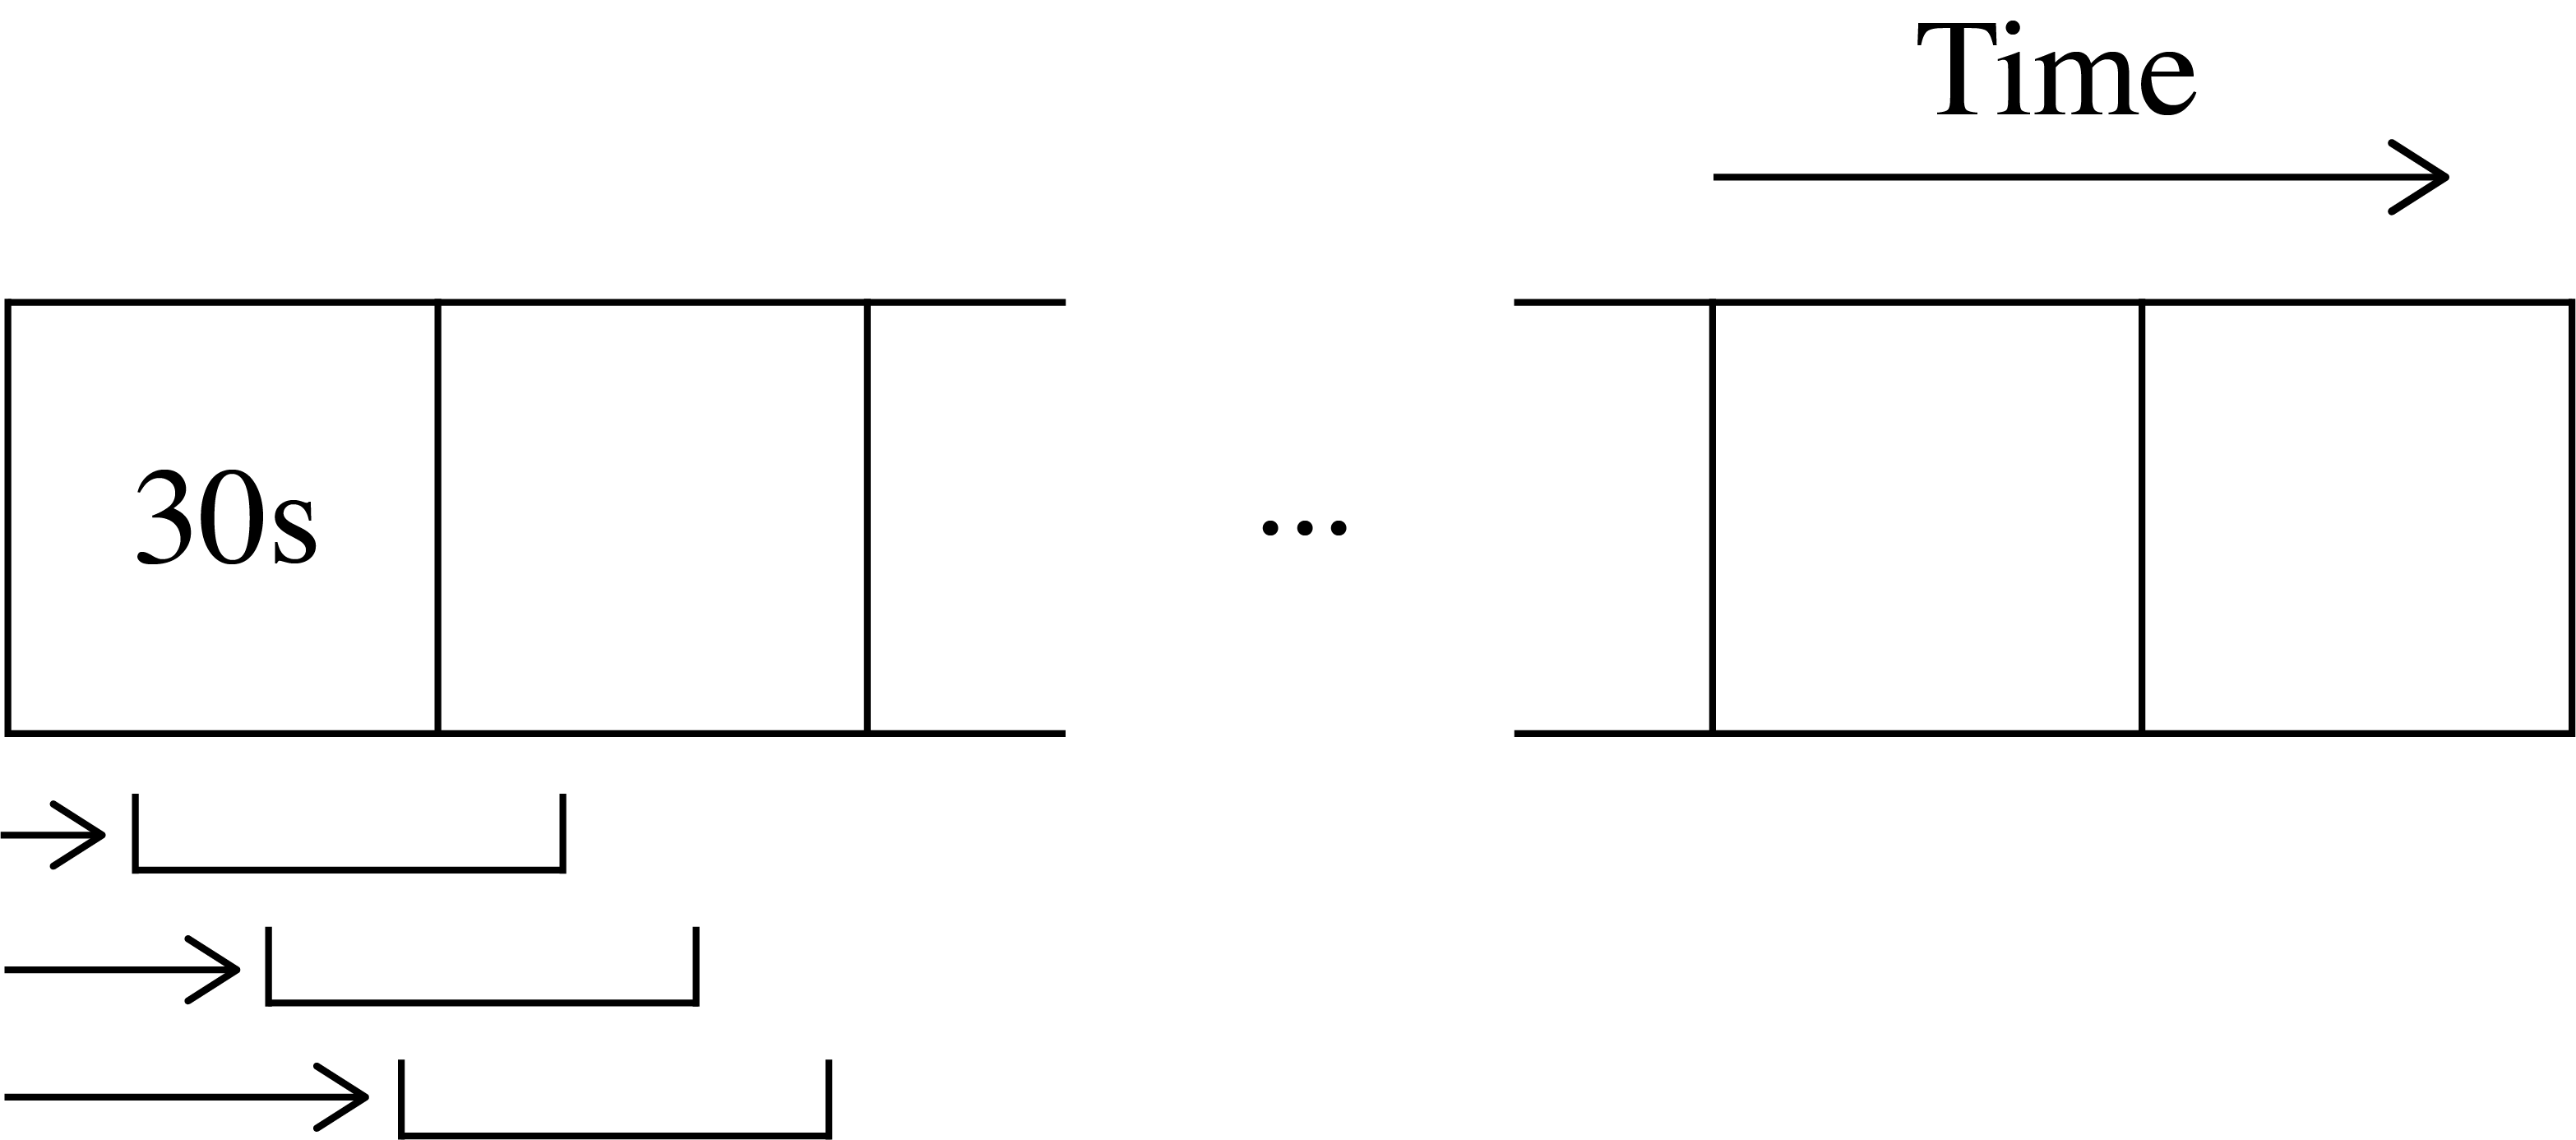
\includegraphics[width=0.8\textwidth]{slidingWindow}
\centering
\caption{Sliding Window technique for synthesizing data spectrogram images}
\label{fig:slidingWindow}
\end{figure}

\begin{figure}[H]
\[ \text{{window\_size}} = \text{{desired\_size}} \times \text{{sampling\_rate}} = 30 \times 256   \]
\caption{Calculate the desired window size. ``desired\_size'' is the length of the windows in seconds. ``sampling\_rate'' is the sampling rate of the recorded data.}
\label{eq:window-size}
\end{figure}


\begin{figure}[H]
\[ \text{{step}} = \frac{{\text{{total\_rows}} - \text{{window\_size}}}}{{\text{{target}} - 1}}  \]
\caption{Calculate the ``step'' or ``speed'' of the sliding window. Can also be described as the offset between window starting points. ``target'' is the desired number of windows.}
\label{eq:step}
\end{figure}

\begin{figure}[H]
\[ \text{{windows}} = \left\{ \left( \lfloor i \times \text{{step}} \rfloor, \lfloor i \times \text{{step}} + \text{{window\_size}} \rfloor \right) \mid i \in \{0, 1, 2, ..., \text{{target}} - 1\} \right\}  \]
\caption{Produces an set of pairs, where an pair describes the start and ending index of an single window. The set length is the same as ``target''}
\label{eq:windows}
\end{figure}

\subsubsection{\acrfull{cnn} and tuning methodology}

\paragraph{Overview}\mbox{}\\

Due to the lack of suitable subjects discussed in \ref{synthesize-data} this project focused on tuning an \acrshort{cnn} and its architecture. The number of convolutional blocks and dense layers, as well as the dense layer's complexity, were setup as the model's architecture tuning variables, this is further disused in \ref{variables} along with the other variables used for tuning. The loss function and optimizer however were not changed between model iterations and were set to Categorical Cross-Entropy and the Adam Optimizer respectively. Categorical Cross Entropy \ref{eq:cat-ce} is a common loss function for multi-class classification applications such as this project, therefore all models within this project utilized the same Categorical Cross Entropy function allowing for the comparison of the loss metrics.

\begin{figure}[H]
\[ H(y, \hat{y}) = -\sum_{i} y_i \log(\hat{y}_i)  \]
\caption{Categorical Cross-Entropy}
\label{eq:cat-ce}
\end{figure}

The Adam optimizer combines two different versions of stochastic gradient descent; Adaptive Gradient Algorithm and Root Mean Square Propagation. Both of these optimizer functions handle the learning rate for each node within a neural network allowing for more efficient training. The two functions manage the learning rates differently with the Adaptive Gradient Algorithm being more applicable for natural language and computer vision problems, Root Mean Square Propagation however suites online learning and non-stationary problems \cite{brownlee2021adam}. Adam combines these two approaches, realizing the benefit of each of them, and configures the learning rates accordingly. The performance of Adam when compared to other optimizer functions can be seen in \ref{fig:adam} \cite{brownlee2021adam}.


\begin{figure}[H]
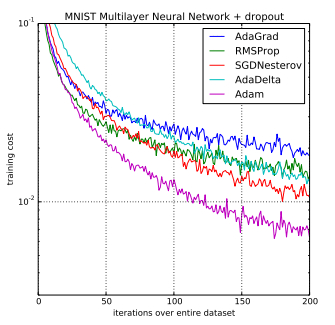
\includegraphics[width=0.6\textwidth]{adam}
\centering
\caption{Optimization function performance comparison.}
\label{fig:adam}
\end{figure}


With only a single machine and the time available specified in \ref{gantt}, applying \acrfull{loocv} for all architecture and variable configurations would have been impossible. Therefore a testing training split ratio needed to be decided on. The time costs of running testing, especially on complex \acrshort{cnn} models were high, consequently, a large split for testing would be impractical as it would further drive up the training testing times. Due to the nature of the way the data was synthesized as well, a smaller testing split would be representative of all the available data for each class, this therefore led the project to use an 80\% training and 20\% testing split. 

\paragraph{Architecture}\mbox{}\\


The \acrshort{cnn} was dynamically built in accordance with the current variable configuration. By default, a single 2-dimensional convolutional block was included with an input shape of $(17\times3841\times2)$ such that the model would accept a 30-second \acrshort{stft} window. This convolutional block had 32 filters with a kernel size of $(3\times3\times3)$. The dynamic convolutional blocks were then built, increasing the number of filters following the formula $32 \times (2^i)$ where $i$ is the convolutional block index. Each convolutional block is followed by a batch normalization, and after all convolutional blocks, a 2 dimensional Max Pooling layer with a pool size of $(2\times2)$ is applied, along with a Flatten layer preparing the data to be passed to the dense layers.

After the convolutional blocks and related layers have been added the dense layers are built. Again, a single dense layer is added by default which has an output shape of $(1, 3)$, preceding this dense layer is the dynamically generated dense layers. These layers have a set output shape specified in the architecture tuning variables.


\begin{lstlisting}[style=pythonstyle, caption={Function which dynamically builds an \acrshort{cnn} model from the specified parameters. Logging has been removed.}, label={lst:compile-model}]
    def compile_model(self, num_conv_layers=4, num_dense_layers=4, dense_layer_size=64):
        self.num_conv_layers = num_conv_layers
        self.num_dense_layers = num_dense_layers 
        self.dense_layer_size = dense_layer_size 

        if num_dense_layers < 1 or num_conv_layers < 0: 
            raise ValueError

        model = models.Sequential()

        # add convolutional layers
        model.add(layers.Conv2D(32, kernel_size=(3, 3), activation='relu', input_shape=(17, 3841, 2)))
        for i in range(1, num_conv_layers):
            model.add(layers.Conv2D(32 * (2**i), kernel_size=(3, 3), activation='relu'))
            model.add(layers.BatchNormalization())

        model.add(layers.MaxPooling2D(pool_size=(2, 2)))
        model.add(layers.Flatten())

        # add dense layers
        for i in range(num_dense_layers-1):
            model.add(layers.Dense(dense_layer_size, activation='relu'))

        model.add(layers.Dense(3, activation='softmax'))
        model.compile(loss='categorical_crossentropy', optimizer='adam', metrics=['accuracy'])
\end{lstlisting}

\paragraph{Tuning Variables}\label{variables}

\ref{tab:variables} shows the different variables and their possible values used for model tuning. A model was trained for possible configurations of these variables.

\begin{table}[H]
\centering
\begin{tabular}{llll}
\multicolumn{4}{l}{Model Parameters}        \\
Num. Conv. Layers    & 2     & 3     &      \\
Num. Dense Layers    & 4     & 8     & 12   \\
Dense Layer Size     & 64    & 128   & 256  \\ 
& & & \\
\multicolumn{4}{l}{Architecture Parameters} \\
Epochs               & 1     & 8     & 32   \\
Batch Size           & 16    & 32    & 48  
\end{tabular}
\caption{The possible values for each tuning variable.}
\label{tab:variables}
\end{table}

The number of convolutional layers had to be limited; as the filter size increased exponentially with each layer an \acrfull{oom} error would occur when the filter size was too large. Therefore only 2 and 3 convolutional layers were tested. The number of epochs was also limited due to training time. With this configuration of tuning variables, 162 models were required to be trained.

\paragraph{Metrics}

For each model, a plain text file was created during its tuning process. This plain text file recorded the start and end times of each process, including its model compiling, model training, and model testing. The file also contained metrics such as the training and testing accuracy and loss, the final confusion matrix, and the normalized confusion matrix. A classification report was also generated which calculated the precision, recall, F1 score, and support for each class. The classification report also calculated the accuracy of the model. An example of this file can be seen in \ref{lst:tuning-metrics}. The results are available along with a discussion in \ref{results}.

\begin{lstlisting}[style=logstyle, caption={Logging file programmatically generated during the tuning process. Training accuracy and loss lines have been trimmed for readability.}, label={lst:tuning-metrics}]
       ---------------------------------------------
                    current configuration

                conv layers count   :   2
                    dense layer count   :   4
                        dense layer size    :   128

                            epochs  :   32
                                batch_size  :   32

            
                
dataset generation start : 2024-04-06 21:00:09.473945
one hot matrix:
['interictal', 'preictal', 'ictal']
{'interictal': 0, 'preictal': 1, 'ictal': 2}
[[1. 0. 0.]
 [0. 1. 0.]
 [0. 0. 1.]]
target subjects : ['chb06']
dataset generation end : 2024-04-06 21:00:09.666774
compiling model start : 2024-04-06 21:00:09.669026
compiling model end : 2024-04-06 21:00:09.847257
training start : 2024-04-06 21:00:09.848724
training end : 2024-04-07 01:59:22.883511
training accuracy: [0.974943995475769, 0.997187077999115, 0.9978642463684082, 0.9973433613777161, 1.0...
training loss: [1.4391484260559082, 0.01381457969546318, 0.019184233620762825, 0.043409526348114014...
saving model start : 2024-04-07 01:59:22.893082
saving model end : 2024-04-07 01:59:34.687428
cmatrix prediction start : 2024-04-07 01:59:34.691563
cmatrix prediction end : 2024-04-07 02:02:52.020467
Confusion Matrix:
[[1626    0    0]
 [   0 1543    0]
 [   0    0 1631]]
Normalized Confusion Matrix:
[[1. 0. 0.]
 [0. 1. 0.]
 [0. 0. 1.]]
Classification Report:
              precision    recall  f1-score   support

  interictal       1.00      1.00      1.00      1626
    preictal       1.00      1.00      1.00      1543
       ictal       1.00      1.00      1.00      1631

    accuracy                           1.00      4800
   macro avg       1.00      1.00      1.00      4800
weighted avg       1.00      1.00      1.00      4800
\end{lstlisting}


\subsubsection{Real Time Simulation}

A real-time simulation was built to show the potential of the preprocessing and prediction pipeline, proving its ability to output a prediction from raw \acrshort{eeg} data each second. The real-time solution was built with ``NiceGui.py'' and the solution to setup model tuning was adapted to work in this new environment, implementing each step as defined above. The NiceGui solution has a hard-coded path to a saved Keras model. This model is loaded before the simulation begins and is used to run the predictions. \ref{fig:real-time} contains an image of the real-time simulation.

\begin{figure}[H]
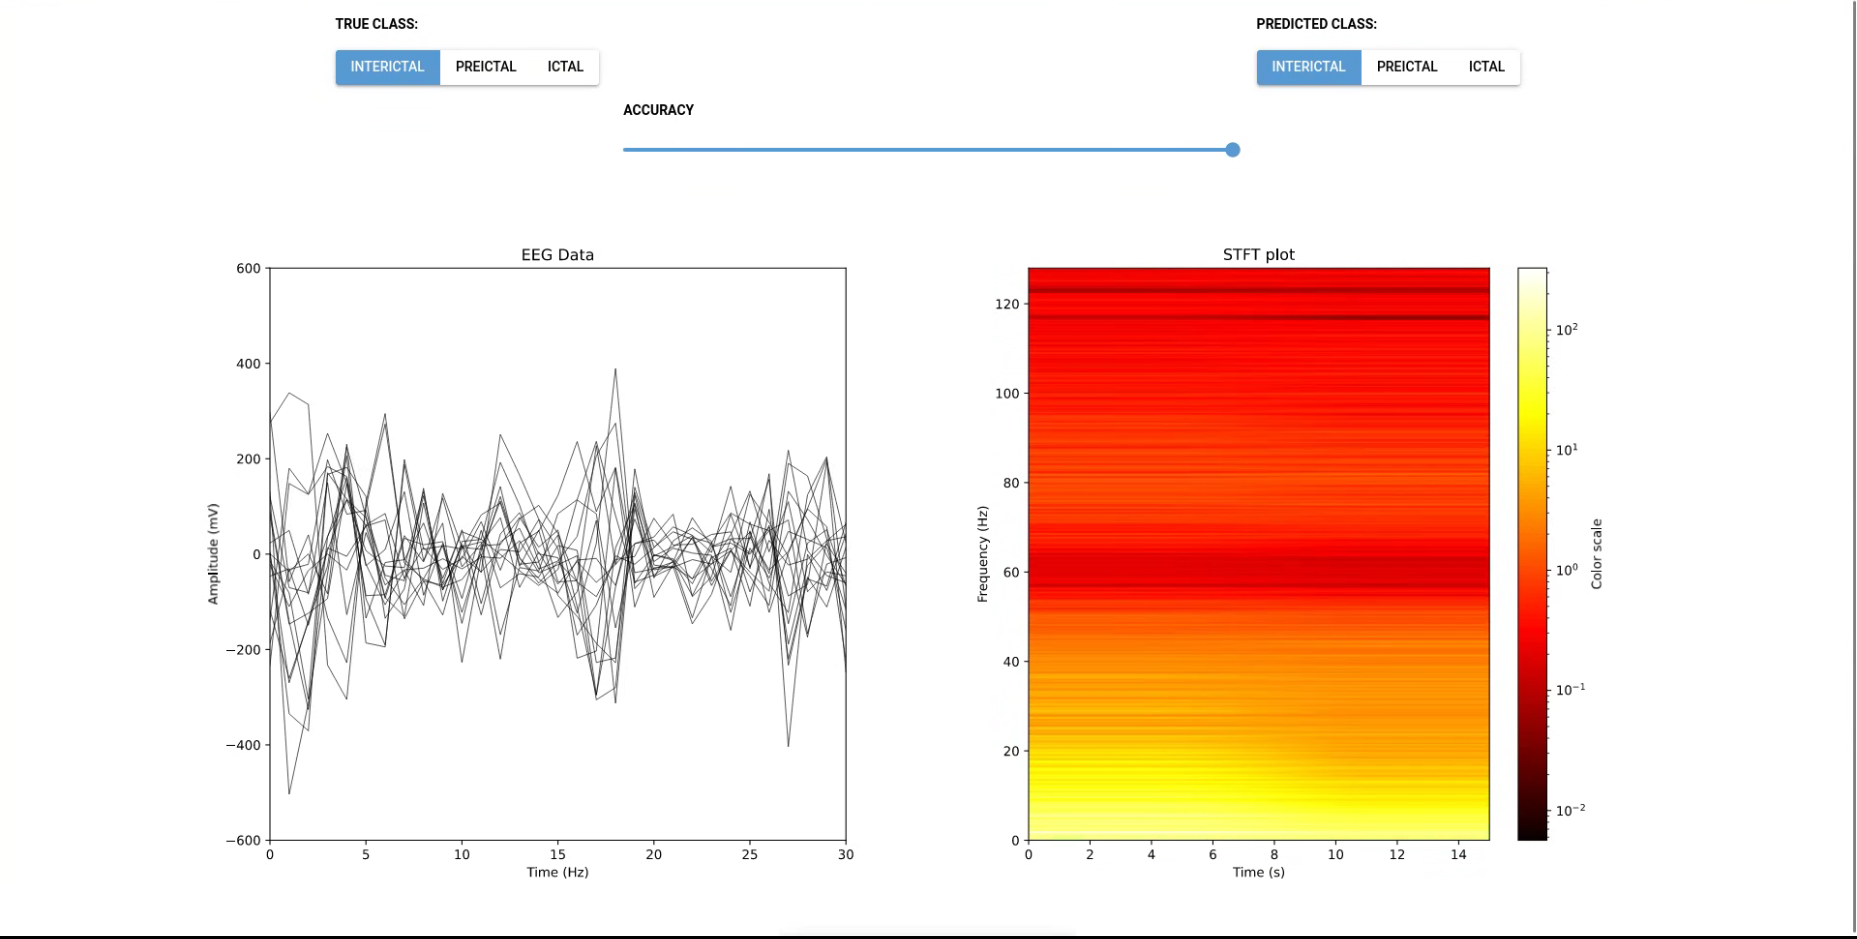
\includegraphics[width=\textwidth]{real-time}
\centering
\caption{Screenshot of running real-time simulation.}
\label{fig:real-time}
\end{figure}

Within the simulation you can toggle which class the \acrshort{eeg} data is being pulled from, this then replaces the last 30 seconds of streamed data with data extracted from the newly selected class. This, in turn, refreshed the two plots on the webpage, with the left plot representing the signals from each \acrshort{eeg} node, and the right plot being the produced \acrshort{stft} window used for prediction. The predicted class then appears in the top right, and the accuracy bar, representing the accuracy as a percentage is updated.


\subsection{Problems Encountered}\label{issues}


There have been many issues faced throughout this project. From the very start managing bodies of datasets would not respond, this impacted my decision-making when selecting one of the datasets discussed in \ref{datasets}. Furthermore, once the \acrshort{chb} dataset was selected there were discrepancies within the summary files, and the extracted data with channel names not matching. The \acrshort{chb} dataset also did not record the \acrshort{eeg} values in the same manner for all subjects, this led to some data points from \acrshort{eeg} nodes to be discarded as those specific \acrshort{eeg} channels were not used for all subjects. On average this meant over 25\% of recorded data had to be removed. Of what was recorded, some subjects had very little data for certain classes with an overabundance of recorded interictal data. Having such little data for certain classes decreases the confidence of the synthesized data, as even though enough data points are available, the synthesized data may not be representative of a real-life situation.

This project's approach changed substantially across its development. Originally development attempted to extract numeric and statistical features for each recorded point, more akin to traditional \acrshort{ann} methodologies, however, this approach was abandoned as it would not have been able to meet the real-time objective of this project.

Tuning the models raised more problems than anything else in this project, with \acrshort{oom} issues being a common problem occurring throughout the model tuning process and the development of the real-time simulation. All code affected with \acrshort{oom} problems had to be carefully re-written to remove any memory leaks as well as implementing generator functions which for example would open the dataset paths used for training only when required. Some \acrshort{oom} errors were not avoidable, however. Certain model architecture configurations would lead to memory errors with convolutional block complexity growing exponentially only a maximum of 3 convolutional blocks were able to be used. Dense layer count and complexity on top also added to the problem.

There were also many failed attempts at tuning the models. A re-occurring error was missing data points or even classes when tuning, this led to many trained models being invalid as they would only predict 2, or even 1 class due to its training data. Even when tuning was seemingly working this issue would appear with no exceptions being raised or problems being apparent. Over 250 trained models \ref{lst:model-list} have been discarded due to this problem alone, this has drastically reduced the results available for discussion.

\section{Review}

\subsection{Objectives and Requirements}



\begin{table}[H]
\centering
\begin{tabular}{p{0.1\textwidth}p{0.7\textwidth}p{0.1\textwidth}}
Index & Objective                                                                                                                                                                                                                    & Achieved \\
1     & Research and find an suitable dataset allowing for the classification of the interictal, preictal, and ictal periods.                                                                                                        & True     \\
2     & Research and find an suitable \acrshort{ml} model approach.                                                                                                                                                                  & True     \\
3     & Create a data preperation and preprocessing pipeline which extracts the dataset into an \acrshort{ml} format suitable for training and testing.                                                                              & True     \\
4     & Undergo parameter tuning and model architecture tuning of the selected \acrshort{ml} model approach.                                                                                                                         & True     \\
5     & Produce a simulation interface which streams \acrshort{eeg} data in real time through the preprocessing pipeline and into the optimal model. The simulation should show the current classification to the user every second. & True    
\end{tabular}
\caption{Objectives taken from \ref{objectives}.}
\label{tab:objectives-review}
\end{table}


\begin{table}[H]
\centering
\begin{tabular}{p{0.1\textwidth}p{0.7\textwidth}p{0.1\textwidth}}
Index & Requirements                                                                               & Achieved \\
1     & Develop and preprocessing pipeline which accepts raw \acrshort{eeg} data.                  & True     \\
2     & Tune an number of models to find the optimal variable configuration.                       & True     \\
3     & Ensure that the optimal model has an accuracy of $\geq90\%$ against an validation dataset. & True     \\
4     & From \acrshort{eeg} data extraction to prediction, the process must take at most 1 second. & True     \\
5     & Create an real-time simulation mimicking an real life application.                         & True    
\end{tabular}
\caption{Requirements taken from \ref{requirements}.}
\label{tab:requirements-review}
\end{table}

The above tables correspond to the items in \ref{requirements} and \ref{objectives}. Upon review, even with the tuning issues discussed in \ref{issues}, this project was able to achieve all of its objectives and requirements.

\subsection{Results}\label{results}




\subsection{Future Advancements}


\subsubsection{Generic Model}

All models have been trained against a single subject's data, this has allowed the \acrshort{cnn} to pick up on their own characteristics for each class. Moving forward, a generic model for all subjects should be trained and evaluated against a single-subject model. Through this evaluation, a definitive answer can be found, pointing towards either a generic model having the same capabilities as a single-subject model or if a model for this application would have to be developed on a per-subject basis.

\subsubsection{\acrshort{eeg} node configuration}

The current model utilizes 17 \acrshort{eeg} nodes which are all positioned on the subject's cranium. In a real-life application reducing the number of \acrshort{eeg} nodes will drastically increase the convenience of having an \acrshort{eeg} based prediction device. Therefore a tuning process, where models are developed with different configurations for all possible \acrshort{eeg} node combinations will need to be developed. Reducing the number of \acrshort{eeg} nodes will also decrease the price of a prediction system along with the chance of a node, and therefore the device failing.

\subsubsection{\acrshort{stft} parameters}

\acrshort{stft} has 2 variables, being the window size and the time step. The window size affects the time and frequency resolution of the final image see \ref{fig:stft2}. The time step defines the distance between two successive windows. Both of these variables should be tuned as a balance of the time and frequency resolution needs to be found to produce optimal results. This will be a lengthy process as different \acrshort{cnn} convolutional block configurations will need to be tested for each \acrshort{stft} parameter combination.



\subsubsection{Model Architecture}

This project attempts to find the optimal \acrshort{cnn} architecture, although due to issues discussed in \ref{issues} not all model architectures were tested. Therefore an approach that tunes the architecture would be beneficial as it may show that a less complex model will have the ability to produce just as successful metrics. Simplifying the model will allow it to run on a small or embedded device, perfect for a prediction system.


\subsubsection{Prediction System}

A prediction system prototype should be created to allow for real-life trials. OpenBCI is a company that produces \acrshort{eeg} devices that can stream data in real-time to a machine. OpenBCI advertises \acrshort{eeg} nodes, microcontrollers, and 3D printed models which hold the components on their website. OpenBCI has also made the STL files for their 3D models accessible through their GitHub \url{https://github.com/OpenBCI/Ultracortex/tree/master/Mark_IV}. Using these materials along with either their microcontroller or a custom one running off open source software such as \url{https://github.com/Pi-EEG/EEGwithRaspberryPI} should allow for an easy platform to create such a prediction device.


\subsubsection{Online Learning}


Due to a lack of datasets for this application, converting the model's training strategy to online learning, along with collecting data in real-time through the prediction system discussed above, will allow for a model to continuously refine itself, picking up on characteristics for that specific subject. This approach, if successful should allow for the highest confidence, with minimal false positives alleviating unneeded stress for the user.


\section{Professional Issues and Risks}

\subsection{Professional Issues}\label{issues}

\begin{enumerate}
    \item Legal Issues:
    \begin{itemize}
        \item If the project was to be implemented into a seizure prediction system then GDPR legislation would have to be upheld; if the model is utilizing online learning then the data being stored will not be anonymous, meaning the data will have to be deleted when required and available to send to the user on their request. If the data however was truly anonymous, akin to the \acrshort{chb} dataset used in this project, then the data does not fall under GDPR.
Another legal issue could arise if a seizure was not predicted correctly leading to a user suing the company producing the prediction system. This could be solved through an agreement that the end user has to accept, stating the producers of the product, including the developers are not liable.
    \end{itemize}
    \item Social Issues:
    \begin{itemize}
    	 \item People from all walks of life have epilepsy, and due to financial costs, some may not be able to afford the prediction system. This will be an issue that may not be solvable by the producers of the software and instead may need to rely on funding such as a governmental body, healthcare service, or charity. The producers can make the software open source allowing users to fit it onto their own hardware, although that will take time, money, and knowledge for the individual to set up an equivalent system.
    \end{itemize}
        \item Ethical Issues:
    \begin{itemize}
    	 \item The final product should attempt to achieve the same accuracy regardless of age or gender, although due to the differences in the way each person's brain functions and its characteristics, this may be a difficult task to achieve. In an ideal world either a generic model would exist, or models would be trained off datasets specific to age or gender allowing for common characteristics between individuals in those groups to be picked up on, however, there is a significant lack of data currently available making this unfeasible.
    \end{itemize}
        \item Environmental Issues:
    \begin{itemize}
    	 \item EEG nodes are comparatively inexpensive to their possible benefits, due to the low price of EEG nodes the creation of a prediction device won't have a large material cost. The \acrshort{ml} model tuning process however will have a large energy cost. This will need to be taken into account when setting up a system that tunes models at an industry scale. Steps will have to be taken to minimize the energy consumption of the system.
    \end{itemize}
            \item Intellectual Property Issues:
    \begin{itemize}
    	 \item There will be an issue when deciding who owns the recorded data. If the company that produces the final product owns it then they can utilize the large amount of data to further refine and train more advanced models, allowing them to tackle other issues such as the ones discussed in ``Social Issues'', although this should be a choice for the end user. Another issue may be patenting the product and which components should or can be patented or copyrighted.
    \end{itemize}
        \item Accessibility Issues:
    \begin{itemize}
    	 \item As discussed epileptic patients come from all walks of life which means the final device needs to have an accessible interface, allowing everyone to have a clear indication of the state of the device, including the preictal period alert or even if the device is on. Different people will need different alert methods, and the final device should be extensible, allowing the final patient to fit it to their disability. Some variants of the device should have any combination of light, sound, and vibration alerts, as well as notifications to any of their other devices. This will allow anyone, regardless of disability to be alerted if a preictal period has been detected.
    \end{itemize}
\end{enumerate}

\subsection{Risks}

\subsubsection{Risk Matrix}

The numbers in each cell of the risk matrix corresponds to the items in \ref{issues}.

\begin{table}[H]
\centering
\begin{tabular}{l|llll}
                              & \multicolumn{4}{l}{Harm Severity}                                                                                                                                                             \\
\multirow{-2}{*}{Probability} & \multicolumn{1}{l|}{Minor}                    & \multicolumn{1}{l|}{Marginal}                 & \multicolumn{1}{l|}{Critical}                 & \multicolumn{1}{l|}{Catastrophic}             \\ \hline
Certain                       & \multicolumn{1}{l|}{\cellcolor[HTML]{FE996B}} & \multicolumn{1}{l|}{\cellcolor[HTML]{FE996B}} & \multicolumn{1}{l|}{\cellcolor[HTML]{FD6864}} & \multicolumn{1}{l|}{\cellcolor[HTML]{FD6864}} \\ \hline
Likely                        & \multicolumn{1}{l|}{\cellcolor[HTML]{FFFE65}} & \multicolumn{1}{l|}{\cellcolor[HTML]{FE996B}} & \multicolumn{1}{l|}{\cellcolor[HTML]{FE996B}} & \multicolumn{1}{l|}{\cellcolor[HTML]{FD6864}} \\ \hline
Possible                      & \multicolumn{1}{l|}{\cellcolor[HTML]{67FD9A}} & \multicolumn{1}{l|}{\cellcolor[HTML]{FFFE65}} & \multicolumn{1}{l|}{\cellcolor[HTML]{FE996B}} & \multicolumn{1}{l|}{\cellcolor[HTML]{FD6864}} \\ \hline
Unlikely                      & \multicolumn{1}{l|}{\cellcolor[HTML]{67FD9A}} & \multicolumn{1}{l|}{\cellcolor[HTML]{FFFE65}} & \multicolumn{1}{l|}{4, 6\cellcolor[HTML]{FFFE65}} & \multicolumn{1}{l|}{3, 5, 7\cellcolor[HTML]{FE996B}} \\ \hline
Rare                          & \multicolumn{1}{l|}{\cellcolor[HTML]{67FD9A}} & \multicolumn{1}{l|}{\cellcolor[HTML]{67FD9A}} & \multicolumn{1}{l|}{\cellcolor[HTML]{FFFE65}} & \multicolumn{1}{l|}{1, 2\cellcolor[HTML]{FFFE65}} \\ \hline
\end{tabular}
\caption{Risk Matrix}
\label{tab:risk-matrix}
\end{table}


\subsubsection{Risk Assessment}




%\begin{table}[H]
%\centering
%\begin{tabular}{p{0.03\linewidth}p{0.3\linewidth}p{0.3\linewidth}p{0.3\linewidth}}
\begin{longtable}{p{0.03\linewidth}p{0.3\linewidth}p{0.3\linewidth}p{0.3\linewidth}}
No. & Risk                                              & Impact                                                      & Mitigation Strategy                                          \\
1 & Personal data could be leaked through an attack   & Fail to adhere to GDPR. Criminal Offence & Implement encryption for data as well as increasing security measures \\
2 & Personal data is leaked by unauthorized employee  & Fail to adhere to GDPR. Criminal Offence& Tighten access controls. Educate employees about password and general security\\
3 & Personal data is leaked by an authorized employee & Fail to adhere to GDPR. Criminal Offence& Employ education techniques stating the importance of adhering to GDPR as well as minimizing access to sensitive data.\\
4 & False Negatives for the individual& End users will be unprepared for their seizures and may be caught in an unfavourable situation depending on reliance on the final product.& Implement cross validation techniques. Request all missed seizures to be logged or automatically detected for further training and inspection. \\
5 & False Positives for the individual& A patient may experience un-needed stress or stop important activities due to false positives. Could have measurable knock on effects for an individual. & False positives should be recorded which will allow for further development of the model.\\
6 & False Negatives in a healthcare environment & Staff may not be prepared for an seizure, increasing reaction times & See ``False Negatives for the individual''\\
7 & False Positives in a healthcare environment & Staff may waste time preparing for a seizure which never occours, where their help may be needed elsewhere & See ``False Positives for the individual'' \\
%\end{tabular}
\caption{Risk Assessment}
\label{tab:risk-assessment}
%\end{table}
\end{longtable}



\section{Conclusion}

\subsection{Objective Review}


\begin{enumerate}
\item \textit{Research and find a suitable dataset allowing for the classification of the interictal, preictal, and ictal periods.} - Two literature reviews were undergone, evaluating 10 possible datasets; outlining where the \acrshort{eeg} nodes were positioned, their placement method, the recording style (continuous or non-continuous), their application, and even their subject type with some datasets evaluated containing canine subjects. This literature review allowed for the \acrshort{chb} dataset to be selected due to its appropriate node placement, recording style, and human-only subjects.
	
	
\item \textit{Research and find an suitable \acrshort{ml} model approach.} - The second literature review successfully researched different preprocessing pipelines along with \acrshort{ml} models, this literature review was crucial in giving an insight into different approaches and which one would fit into a real-time application. Without these two literature reviews the project would have met serious issues when attempting to meet the accuracy and real-time requirements of this project.
	
	
\item \textit{Create a data preparation and preprocessing pipeline that extracts the dataset into an \acrshort{ml} format suitable for training and testing. } - The pipeline was successfully implemented by using an \acrshort{stft} function along with a notch filter to remove interference. This approach was influenced by the \acrshort{ml} model literature review. This pipeline was chosen as the number of extracted features, steps, and compute-heavy functions was low, giving it the best chance to meet the real-time requirement. The \acrshort{stft} window exceeded expectations and fully meets this requirement, allowing for effective, but fast preprocessing.
        
        
\item \textit{Undergo parameter tuning and model architecture tuning of the selected \acrshort{ml} model approach.} - For tuning \acrshort{ml} models the classes had to be balanced. The chosen approach was to synthesize data by using a sliding window technique, this was used to generate windows until all 3 classes had an equal number of data points. Once the data has been synthesized the pre-processing pipeline was then applied, generating thousands of spectrogram images. Through the use of ``sklearn'', ``Tensorflow'', and ``Keras'' these spectrograms could then be loaded and used for tuning, testing or running a real-time simulation. The tuning process however was slightly buggy, and with more time available this hopefully would of been resolved allowing for a greater number of models to be trained and evaluated. Nevertheless, the results obtained through the tuning process also exceeded my expectations with testing results being near perfect for all tuned models.
        
        
\item \textit{Produce a simulation interface which streams \acrshort{eeg} data in real-time through the preprocessing pipeline and into the optimal model. The simulation should show the current classification to the user every second.} - The developed simulation proves the pipeline's ability to run in real-time which confirms that the project has met the real-time requirement. The simulation streams 17x256 data points each second for the currently selected class and produces a prediction using a trained model. In the future, this simulation can be easily modified to accept real recorded data from a physical \acrshort{eeg} setup. This is discussed in \ref{future-advancements}. At the beginning of this project, this integration was going to be incorporated into the requirements, however after evaluating the time given it was dropped.
\end{enumerate}

\subsection{Final Thoughts}

This project has successfully achieved all requirements and objectives, producing the groundwork for a successful seizure prediction system. It's proved that the technology has the ability to accurately classify seizure periods, and predict seizures up to 20 minutes before they begin. If a detection system was to be developed it would alleviate large amounts of stress in the day-to-day lives of epileptic patients, something which would be invaluable for them. Even with this groundwork, there are still a lot of developments that can be done, however even with the state of the current project, if a prediction system was to be based on this paper it would be able to exceed expectations and even change the way people go about their day to day lives.

\pagebreak
\section{Bibliography}
\bibliographystyle{agsm}
\bibliography{references}
\pagebreak

\appendix

\section{Links}

\subsection{GitHub}

\url{https://github.com/N3utra1/COMP6013_Dissertation}

\subsection{Video Demonstration}

\url{https://drive.google.com/file/d/1VGSPdRVlAAZp02pIs3qw4FANiYk2peBG/view?usp=sharing}


\section{Results}


Model key: [convolution block count].[dense layer count].[dense layer size]/[batch size].[epochs]


\subsection{Tables}


\begin{table}[H]
\centering
\begin{tabular}{llll}
Model & Training & Testing & Total \\
  2.4.128/16.1    &      0:09:34.252395       &     0:02:29.318160       &     0:12:16.936242        \\
  2.4.128/16.32    &      4:55:14.648736       &     0:02:36.181157       &     4:58:03.207583        \\
  2.4.128/16.8    &      1:13:53.250455       &     0:02:28.278624       &     1:16:34.098996        \\
  2.4.128/32.1    &      0:10:16.908274       &     0:02:58.134548       &     0:13:27.358200        \\
  2.4.128/32.32    &      4:59:13.034787       &     0:03:17.328904       &     5:02:42.546522        \\
  2.4.128/32.8    &      1:21:12.806743       &     0:02:50.145996       &     1:24:15.803703        \\
  2.4.128/48.1    &      0:10:53.791005       &     0:02:57.700320       &     0:14:06.449949        \\
  2.4.128/48.32    &      5:04:12.389344       &     0:02:40.036783       &     5:06:58.710978        \\
  2.4.128/48.8    &      1:21:59.435414       &     0:02:31.724462       &     1:24:43.405594        \\
  2.4.64/16.1    &      0:09:16.671517       &     0:02:20.833553       &     0:11:43.794613        \\
  2.4.64/16.32    &      4:49:23.103991       &     0:02:40.019918       &     4:52:09.480089        \\
  2.4.64/16.8    &      1:18:51.356595       &     0:02:55.648672       &     1:21:53.885149        \\
  2.4.64/32.1    &      0:09:53.286427       &     0:02:30.918573       &     0:12:30.448678        \\
  2.4.64/32.32    &      5:01:06.399645       &     0:03:07.540450       &     5:04:20.224694        \\
  2.4.64/32.8    &      1:21:48.011924       &     0:02:32.670039       &     1:24:27.044614        \\
  2.4.64/48.1    &      0:09:58.299346       &     0:02:59.123882       &     0:13:03.698828        \\
  2.4.64/48.32    &      5:04:12.389344       &     0:02:40.036783       &     5:06:58.710978        \\
  2.4.64/48.8    &      1:20:23.212631       &     0:02:46.982105       &     1:23:16.378890        \\
\end{tabular}
\caption{Time duration metrics for each model in format \%H:\%M:\%S.\%f.}
\label{tab:my-table}
\end{table}




\begin{table}[H]
\centering
\begin{tabular}{lll}
Model & Training Accuracy & Training Loss \\
  2.4.128/16.1    &      0.9832265377044678       &     0.8224268555641174 \\
  2.4.128/16.32    &      0.9993602503091097       &     0.02814496521023102 \\
  2.4.128/16.8    &      0.9976428672671318       &     0.11281578045975693 \\
  2.4.128/32.1    &      0.975464940071106       &     1.4378010034561157 \\
  2.4.128/32.32    &      0.9989679381251335       &     0.04745509265126133 \\
  2.4.128/32.8    &      0.9962754622101784       &     0.18717686411091886 \\
  2.4.128/48.1    &      0.9669219255447388       &     2.318654775619507 \\
  2.4.128/48.8    &      0.9958652406930923       &     0.2898520281258925 \\
  2.4.64/16.1    &      0.9799447655677795       &     0.6853911876678467 \\
  2.4.64/16.32    &      0.9992593247443438       &     0.024666143968849415 \\
  2.4.64/16.8    &      0.9969331100583076       &     0.08956567873635081 \\
  2.4.64/32.1    &      0.9619211554527283       &     1.725386619567871 \\
  2.4.64/32.32    &      0.9987660832703114       &     0.05414362490514908 \\
  2.4.64/32.8    &      0.9953247904777527       &     0.21542102738881397 \\
  2.4.64/48.1    &      0.9655154347419739       &     2.379462718963623 \\
  2.4.64/48.32    &      0.9989125896245241       &     0.07438817310655671 \\
  2.4.64/48.8    &      0.994374118745327       &     0.31704871635884047 \\
\end{tabular}
\caption{Accuracy and Loss metrics (average across epochs) during model training.}
\label{tab:training-metrics}
\end{table}





\begin{table}[H]
\centering
\begin{tabular}{ll}
Model & Testing Accuracy \\
  2.4.128/16.1    &      0.99   \\
  2.4.128/16.32    &      1.00   \\
  2.4.128/16.8    &      1.00   \\
  2.4.128/32.1    &      1.00   \\
  2.4.128/32.32    &      1.00   \\
  2.4.128/32.8    &      1.00   \\
  2.4.128/48.1    &      1.00   \\
  2.4.128/48.8    &      1.00   \\
  2.4.64/16.1    &      1.00   \\
  2.4.64/16.32    &      1.00   \\
  2.4.64/16.8    &      1.00   \\
  2.4.64/32.1    &      1.00   \\
  2.4.64/32.32    &      1.00   \\
  2.4.64/32.8    &      1.00   \\
  2.4.64/48.1    &      1.00   \\
  2.4.64/48.32    &      1.00   \\
  2.4.64/48.8    &      1.00   \\
\end{tabular}
\caption{Accuracy metrics obtained during testing.}
\label{tab:testing-accuracy}
\end{table}

\pagebreak


\begin{longtable}{llll}
Model                    & \multicolumn{3}{l}{Confusion Matrix} \\
\multirow{3}{*}{2.4.128/16.1}   &  1593 & 33 & 0 \\
                                                                            &  0 & 1543 & 0 \\
                                                                            &  0 & 0 & 1631 \\ \hline
\multirow{3}{*}{2.4.128/16.32}   &  1626 & 0 & 0 \\
                                                                            &  0 & 1543 & 0 \\
                                                                            &  0 & 0 & 1631 \\ \hline
\multirow{3}{*}{2.4.128/16.8}   &  1625 & 1 & 0 \\
                                                                            &  0 & 1543 & 0 \\
                                                                            &  0 & 0 & 1631 \\ \hline
\multirow{3}{*}{2.4.128/32.1}   &  1626 & 0 & 0 \\
                                                                            &  0 & 1543 & 0 \\
                                                                            &  0 & 0 & 1631 \\ \hline
\multirow{3}{*}{2.4.128/32.32}   &  1626 & 0 & 0 \\
                                                                            &  0 & 1543 & 0 \\
                                                                            &  0 & 0 & 1631 \\ \hline
\multirow{3}{*}{2.4.128/32.8}   &  1626 & 0 & 0 \\
                                                                            &  0 & 1543 & 0 \\
                                                                            &  0 & 0 & 1631 \\ \hline
\multirow{3}{*}{2.4.128/48.1}   &  1626 & 0 & 0 \\
                                                                            &  0 & 1543 & 0 \\
                                                                            &  0 & 0 & 1631 \\ \hline
\multirow{3}{*}{2.4.128/48.8}   &  1626 & 0 & 0 \\
                                                                            &  0 & 1543 & 0 \\
                                                                            &  0 & 0 & 1631 \\ \hline
\multirow{3}{*}{2.4.64/16.1}   &  1626 & 0 & 0 \\
                                                                            &  0 & 1543 & 0 \\
                                                                            &  0 & 0 & 1631 \\ \hline
\multirow{3}{*}{2.4.64/16.32}   &  1626 & 0 & 0 \\
                                                                            &  0 & 1543 & 0 \\
                                                                            &  0 & 0 & 1631 \\ \hline
\multirow{3}{*}{2.4.64/16.8}   &  1626 & 0 & 0 \\
                                                                            &  0 & 1543 & 0 \\
                                                                            &  0 & 0 & 1631 \\ \hline
\multirow{3}{*}{2.4.64/32.1}   &  1626 & 0 & 0 \\
                                                                            &  5 & 1538 & 0 \\
                                                                            &  0 & 0 & 1631 \\ \hline
\multirow{3}{*}{2.4.64/32.32}   &  1626 & 0 & 0 \\
                                                                            &  0 & 1543 & 0 \\
                                                                            &  0 & 0 & 1631 \\ \hline
\multirow{3}{*}{2.4.64/32.8}   &  1626 & 0 & 0 \\
                                                                            &  0 & 1543 & 0 \\
                                                                            &  0 & 0 & 1631 \\ \hline
\multirow{3}{*}{2.4.64/48.1}   &  1626 & 0 & 0 \\
                                                                            &  0 & 1543 & 0 \\
                                                                            &  0 & 0 & 1631 \\ \hline
\multirow{3}{*}{2.4.64/48.32}   &  1626 & 0 & 0 \\
                                                                            &  0 & 1543 & 0 \\
                                                                            &  0 & 0 & 1631 \\ \hline
\multirow{3}{*}{2.4.64/48.8}   &  1626 & 0 & 0 \\
                                                                            &  0 & 1543 & 0 \\
                                                                            &  0 & 0 & 1631 \\ 
\caption{Generated Confusion Matrix during the model tuning process.}
\label{tab:cmatrix}
\end{longtable}

\pagebreak

\begin{longtable}{llll}
Model                    & \multicolumn{3}{l}{Normalized Confusion Matrix} \\ 
\multirow{3}{*}{2.4.128/16.1}   &  1.0 & 0.02093909 & 0.0 \\
                                                                            &  0.0 & 0.97906091 & 0.0 \\
                                                                            &  0.0 & 0.0 & 1.0 \\ \hline
\multirow{3}{*}{2.4.128/16.32}   &  1.0 & 0.0 & 0.0 \\
                                                                            &  0.0 & 1.0 & 0.0 \\
                                                                            &  0.0 & 0.0 & 1.0 \\ \hline
\multirow{3}{*}{2.4.128/16.8}   &  1.0 & 0.000647668394 & 0.0 \\
                                                                            &  0.0 & 0.999352332 & 0.0 \\
                                                                            &  0.0 & 0.0 & 1.0 \\ \hline
\multirow{3}{*}{2.4.128/32.1}   &  1.0 & 0.0 & 0.0 \\
                                                                            &  0.0 & 1.0 & 0.0 \\
                                                                            &  0.0 & 0.0 & 1.0 \\ \hline
\multirow{3}{*}{2.4.128/32.32}   &  1.0 & 0.0 & 0.0 \\
                                                                            &  0.0 & 1.0 & 0.0 \\
                                                                            &  0.0 & 0.0 & 1.0 \\ \hline
\multirow{3}{*}{2.4.128/32.8}   &  1.0 & 0.0 & 0.0 \\
                                                                            &  0.0 & 1.0 & 0.0 \\
                                                                            &  0.0 & 0.0 & 1.0 \\ \hline
\multirow{3}{*}{2.4.128/48.1}   &  1.0 & 0.0 & 0.0 \\
                                                                            &  0.0 & 1.0 & 0.0 \\
                                                                            &  0.0 & 0.0 & 1.0 \\ \hline
\multirow{3}{*}{2.4.128/48.8}   &  1.0 & 0.0 & 0.0 \\
                                                                            &  0.0 & 1.0 & 0.0 \\
                                                                            &  0.0 & 0.0 & 1.0 \\ \hline
\multirow{3}{*}{2.4.64/16.1}   &  1.0 & 0.0 & 0.0 \\
                                                                            &  0.0 & 1.0 & 0.0 \\
                                                                            &  0.0 & 0.0 & 1.0 \\ \hline
\multirow{3}{*}{2.4.64/16.32}   &  1.0 & 0.0 & 0.0 \\
                                                                            &  0.0 & 1.0 & 0.0 \\
                                                                            &  0.0 & 0.0 & 1.0 \\ \hline
\multirow{3}{*}{2.4.64/16.8}   &  1.0 & 0.0 & 0.0 \\
                                                                            &  0.0 & 1.0 & 0.0 \\
                                                                            &  0.0 & 0.0 & 1.0 \\ \hline
\multirow{3}{*}{2.4.64/32.1}   &  0.9969344 & 0.0 & 0.0 \\
                                                                            &  0.0030656 & 1.0 & 0.0 \\
                                                                            &  0.0 & 0.0 & 1.0 \\ \hline
\multirow{3}{*}{2.4.64/32.32}   &  1.0 & 0.0 & 0.0 \\
                                                                            &  0.0 & 1.0 & 0.0 \\
                                                                            &  0.0 & 0.0 & 1.0 \\ \hline
\multirow{3}{*}{2.4.64/32.8}   &  1.0 & 0.0 & 0.0 \\
                                                                            &  0.0 & 1.0 & 0.0 \\
                                                                            &  0.0 & 0.0 & 1.0 \\ \hline
\multirow{3}{*}{2.4.64/48.1}   &  1.0 & 0.0 & 0.0 \\
                                                                            &  0.0 & 1.0 & 0.0 \\
                                                                            &  0.0 & 0.0 & 1.0 \\ \hline
\multirow{3}{*}{2.4.64/48.32}   &  1.0 & 0.0 & 0.0 \\
                                                                            &  0.0 & 1.0 & 0.0 \\
                                                                            &  0.0 & 0.0 & 1.0 \\ \hline
\multirow{3}{*}{2.4.64/48.8}   &  1.0 & 0.0 & 0.0 \\
                                                                            &  0.0 & 1.0 & 0.0 \\
                                                                            &  0.0 & 0.0 & 1.0 \\ 
\caption{Generated Normalized Confusion Matrix during the model tuning process.}
\label{tab:normed-cmatrix}
\end{longtable}



\begin{table}[H]
\centering
\begin{tabular}{llllll}
Model & Interictal & Preictal & Ictal & Macro Average & Weighted Average \\
 2.4.128/16.1 & 0.99 & 0.99 & 1.00 & 0.99 & 0.99 \\
 2.4.128/16.32 & 1.00 & 1.00 & 1.00 & 1.00 & 1.00 \\
 2.4.128/16.8 & 1.00 & 1.00 & 1.00 & 1.00 & 1.00 \\
 2.4.128/32.1 & 1.00 & 1.00 & 1.00 & 1.00 & 1.00 \\
 2.4.128/32.32 & 1.00 & 1.00 & 1.00 & 1.00 & 1.00 \\
 2.4.128/32.8 & 1.00 & 1.00 & 1.00 & 1.00 & 1.00 \\
 2.4.128/48.1 & 1.00 & 1.00 & 1.00 & 1.00 & 1.00 \\
 2.4.128/48.8 & 1.00 & 1.00 & 1.00 & 1.00 & 1.00 \\
 2.4.64/16.1 & 1.00 & 1.00 & 1.00 & 1.00 & 1.00 \\
 2.4.64/16.32 & 1.00 & 1.00 & 1.00 & 1.00 & 1.00 \\
 2.4.64/16.8 & 1.00 & 1.00 & 1.00 & 1.00 & 1.00 \\
 2.4.64/32.1 & 1.00 & 1.00 & 1.00 & 1.00 & 1.00 \\
 2.4.64/32.32 & 1.00 & 1.00 & 1.00 & 1.00 & 1.00 \\
 2.4.64/32.8 & 1.00 & 1.00 & 1.00 & 1.00 & 1.00 \\
 2.4.64/48.1 & 1.00 & 1.00 & 1.00 & 1.00 & 1.00 \\
 2.4.64/48.32 & 1.00 & 1.00 & 1.00 & 1.00 & 1.00 \\
 2.4.64/48.8 & 1.00 & 1.00 & 1.00 & 1.00 & 1.00 \\
\end{tabular}
\caption{F1 metrics obtained during testing.}
\label{tab:f1-metrics}
\end{table}




\begin{table}[H]
\centering
\begin{tabular}{llllll}
Model & Interictal & Preictal & Ictal & Macro Average & Weighted Average \\
 2.4.128/16.1 & 1.00 & 0.98 & 1.00 & 0.99 & 0.99 \\
 2.4.128/16.32 & 1.00 & 1.00 & 1.00 & 1.00 & 1.00 \\
 2.4.128/16.8 & 1.00 & 1.00 & 1.00 & 1.00 & 1.00 \\
 2.4.128/32.1 & 1.00 & 1.00 & 1.00 & 1.00 & 1.00 \\
 2.4.128/32.32 & 1.00 & 1.00 & 1.00 & 1.00 & 1.00 \\
 2.4.128/32.8 & 1.00 & 1.00 & 1.00 & 1.00 & 1.00 \\
 2.4.128/48.1 & 1.00 & 1.00 & 1.00 & 1.00 & 1.00 \\
 2.4.128/48.8 & 1.00 & 1.00 & 1.00 & 1.00 & 1.00 \\
 2.4.64/16.1 & 1.00 & 1.00 & 1.00 & 1.00 & 1.00 \\
 2.4.64/16.32 & 1.00 & 1.00 & 1.00 & 1.00 & 1.00 \\
 2.4.64/16.8 & 1.00 & 1.00 & 1.00 & 1.00 & 1.00 \\
 2.4.64/32.1 & 1.00 & 1.00 & 1.00 & 1.00 & 1.00 \\
 2.4.64/32.32 & 1.00 & 1.00 & 1.00 & 1.00 & 1.00 \\
 2.4.64/32.8 & 1.00 & 1.00 & 1.00 & 1.00 & 1.00 \\
 2.4.64/48.1 & 1.00 & 1.00 & 1.00 & 1.00 & 1.00 \\
 2.4.64/48.32 & 1.00 & 1.00 & 1.00 & 1.00 & 1.00 \\
 2.4.64/48.8 & 1.00 & 1.00 & 1.00 & 1.00 & 1.00 \\
\end{tabular}
\caption{Precision metrics obtained during testing.}
\label{tab:precision-metrics}
\end{table}




\begin{table}[H]
\centering
\begin{tabular}{llllll}
Model & Interictal & Preictal & Ictal & Macro Average & Weighted Average \\
 2.4.128/16.1 & 0.98 & 1.00 & 1.00 & 0.99 & 0.99 \\
 2.4.128/16.32 & 1.00 & 1.00 & 1.00 & 1.00 & 1.00 \\
 2.4.128/16.8 & 1.00 & 1.00 & 1.00 & 1.00 & 1.00 \\
 2.4.128/32.1 & 1.00 & 1.00 & 1.00 & 1.00 & 1.00 \\
 2.4.128/32.32 & 1.00 & 1.00 & 1.00 & 1.00 & 1.00 \\
 2.4.128/32.8 & 1.00 & 1.00 & 1.00 & 1.00 & 1.00 \\
 2.4.128/48.1 & 1.00 & 1.00 & 1.00 & 1.00 & 1.00 \\
 2.4.128/48.8 & 1.00 & 1.00 & 1.00 & 1.00 & 1.00 \\
 2.4.64/16.1 & 1.00 & 1.00 & 1.00 & 1.00 & 1.00 \\
 2.4.64/16.32 & 1.00 & 1.00 & 1.00 & 1.00 & 1.00 \\
 2.4.64/16.8 & 1.00 & 1.00 & 1.00 & 1.00 & 1.00 \\
 2.4.64/32.1 & 1.00 & 1.00 & 1.00 & 1.00 & 1.00 \\
 2.4.64/32.32 & 1.00 & 1.00 & 1.00 & 1.00 & 1.00 \\
 2.4.64/32.8 & 1.00 & 1.00 & 1.00 & 1.00 & 1.00 \\
 2.4.64/48.1 & 1.00 & 1.00 & 1.00 & 1.00 & 1.00 \\
 2.4.64/48.32 & 1.00 & 1.00 & 1.00 & 1.00 & 1.00 \\
 2.4.64/48.8 & 1.00 & 1.00 & 1.00 & 1.00 & 1.00 \\
\end{tabular}
\caption{Recall metrics obtained during testing.}
\label{tab:recall-metrics}
\end{table}






\subsection{Plots}

\subsubsection{Timings}

\begin{figure}[H]
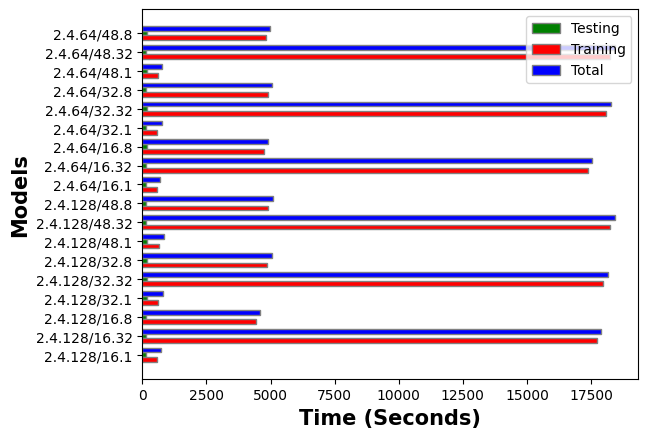
\includegraphics[width=\textwidth]{timings}
\centering
\caption{Recorded time metrics.}
\label{fig:time-metrics}
\end{figure}


\subsubsection{Training Loss}

\begin{figure}[H]
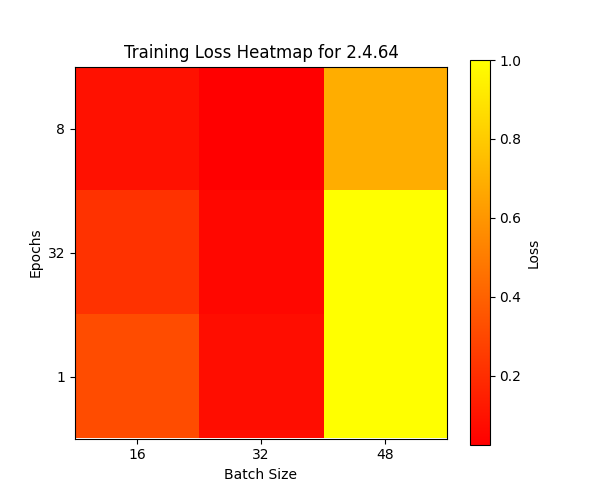
\includegraphics[width=\textwidth]{heatmap_training_loss_2.4.64}
\centering
\caption{Heatmap of loss during training for models with architecture 2.4.64.}
\label{fig:time-metrics}
\end{figure}

\begin{figure}[H]
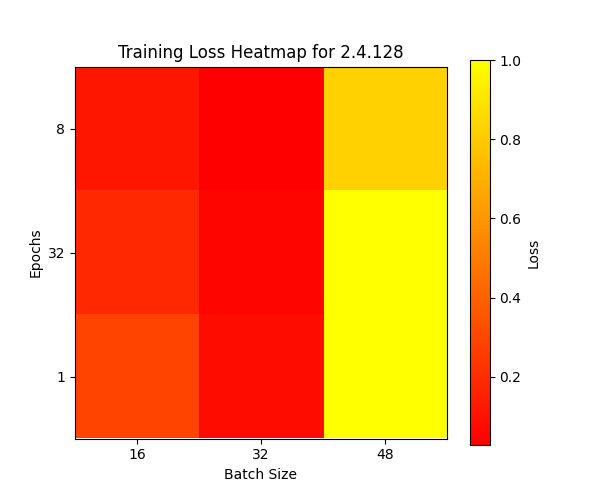
\includegraphics[width=\textwidth]{heatmap_training_loss_2.4.128}
\centering
\caption{Heatmap of loss during training for models with architecture 2.4.128}
\label{fig:time-metrics}
\end{figure}


\subsubsection{Training Accuracy}

\begin{figure}[H]
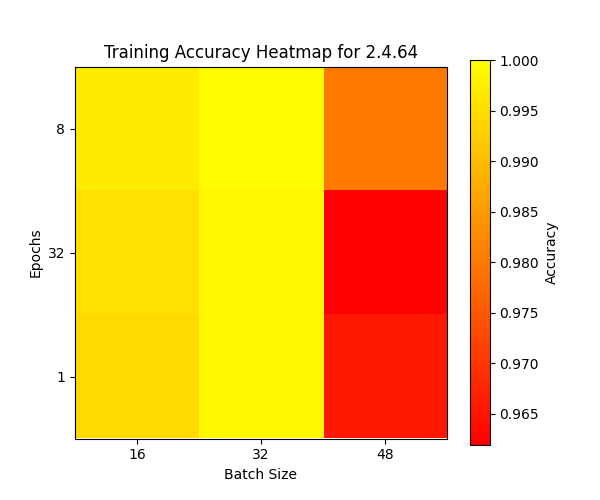
\includegraphics[width=\textwidth]{heatmap_training_accuracy_2.4.64}
\centering
\caption{Heatmap of accuracy during training for models with architecture 2.4.64.}
\label{fig:time-metrics}
\end{figure}

\begin{figure}[H]
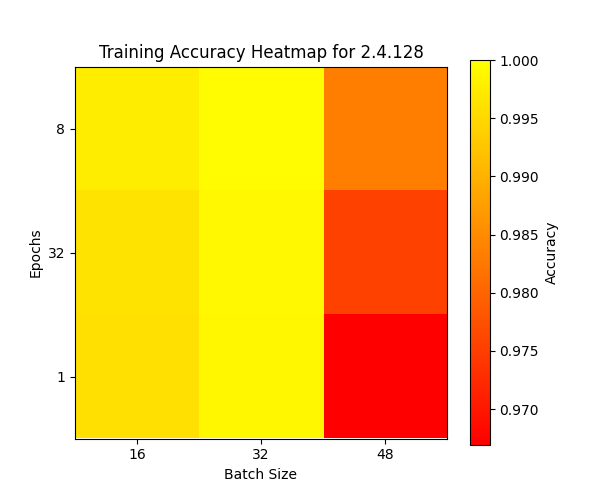
\includegraphics[width=\textwidth]{heatmap_training_accuracy_2.4.128}
\centering
\caption{Heatmap of accuracy during training for models with architecture 2.4.128}
\label{fig:time-metrics}
\end{figure}



\subsubsection{Testing Accuracy}

\begin{figure}[H]
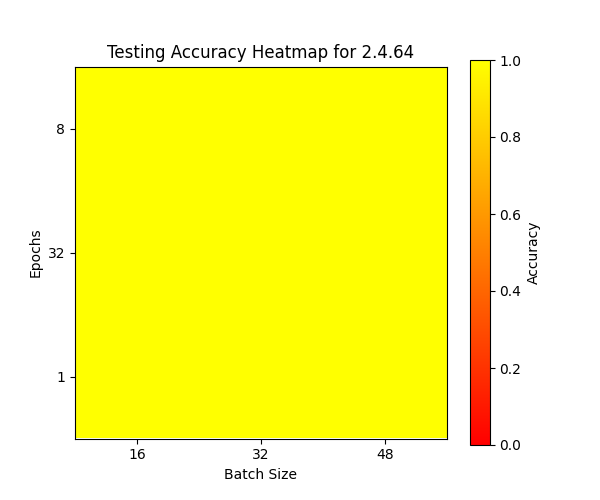
\includegraphics[width=\textwidth]{heatmap_testing_accuracy_2.4.64}
\centering
\caption{Heatmap of accuracy during testing for models with architecture 2.4.64.}
\label{fig:time-metrics}
\end{figure}

\begin{figure}[H]
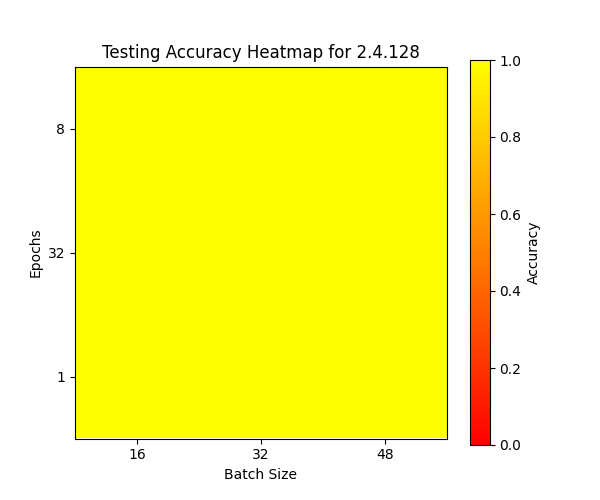
\includegraphics[width=\textwidth]{heatmap_testing_accuracy_2.4.128}
\centering
\caption{Heatmap of accuracy during testing for models with architecture 2.4.128}
\label{fig:time-metrics}
\end{figure}


\subsubsection{Testing Recall}

\begin{figure}[H]
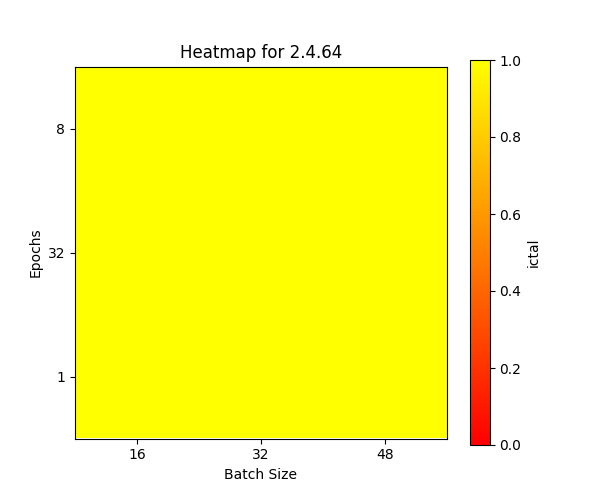
\includegraphics[width=\textwidth]{heatmap_recall_ictal_2.4.64}
\centering
\caption{Heatmap of recall for ictal class during testing for models with architecture 2.4.64.}
\label{fig:time-metrics}
\end{figure}

\begin{figure}[H]
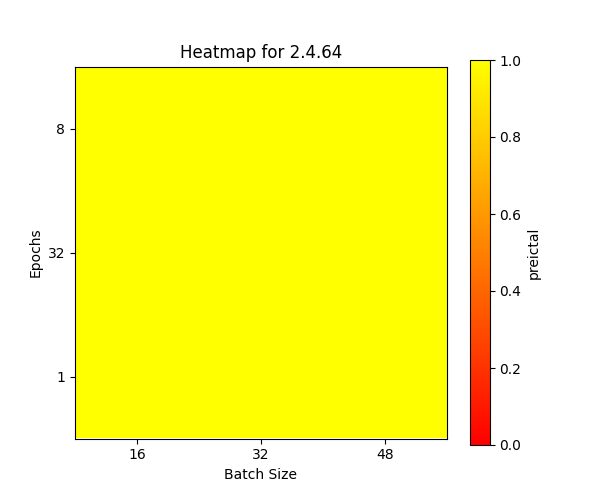
\includegraphics[width=\textwidth]{heatmap_recall_preictal_2.4.64}
\centering
\caption{Heatmap of recall for preictal class during testing for models with architecture 2.4.64.}
\label{fig:time-metrics}
\end{figure}

\begin{figure}[H]
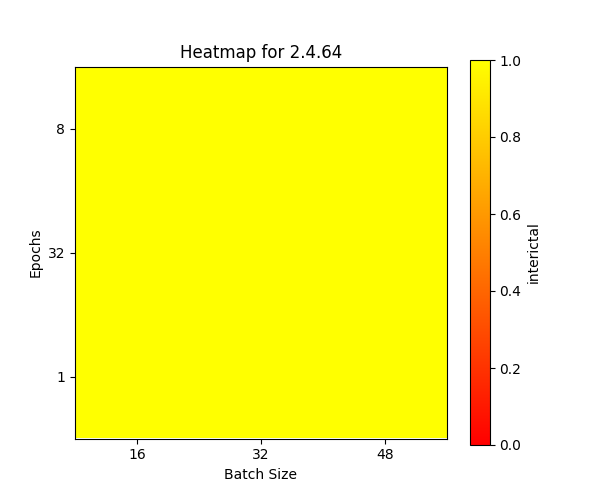
\includegraphics[width=\textwidth]{heatmap_recall_interictal_2.4.64}
\centering
\caption{Heatmap of recall for interictal class during testing for models with architecture 2.4.64.}
\label{fig:time-metrics}
\end{figure}

\begin{figure}[H]
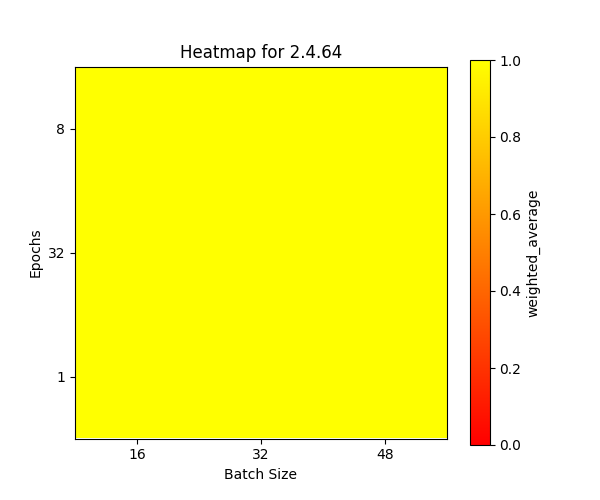
\includegraphics[width=\textwidth]{heatmap_recall_weighted_average_2.4.64}
\centering
\caption{Heatmap of recall (weighted average) during testing for models with architecture 2.4.64.}
\label{fig:time-metrics}
\end{figure}

\begin{figure}[H]
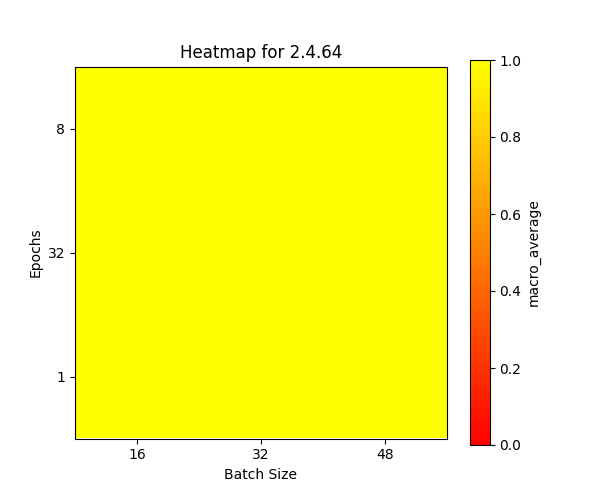
\includegraphics[width=\textwidth]{heatmap_recall_macro_average_2.4.64}
\centering
\caption{Heatmap of recall (macro average) during testing for models with architecture 2.4.64.}
\label{fig:time-metrics}
\end{figure}


\begin{figure}[H]
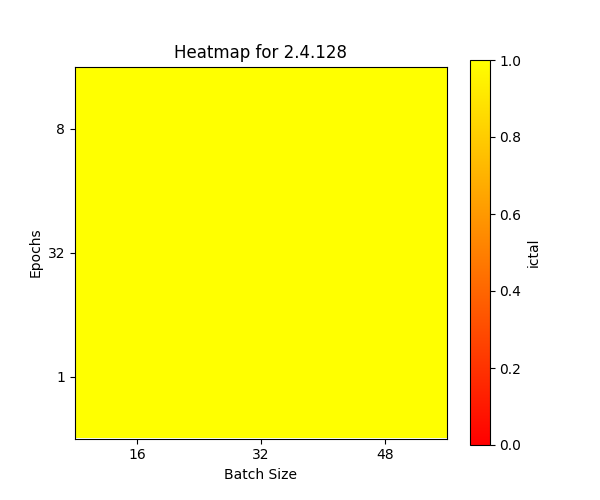
\includegraphics[width=\textwidth]{heatmap_recall_ictal_2.4.128}
\centering
\caption{Heatmap of recall for ictal class during testing for models with architecture 2.4.128.}
\label{fig:time-metrics}
\end{figure}

\begin{figure}[H]
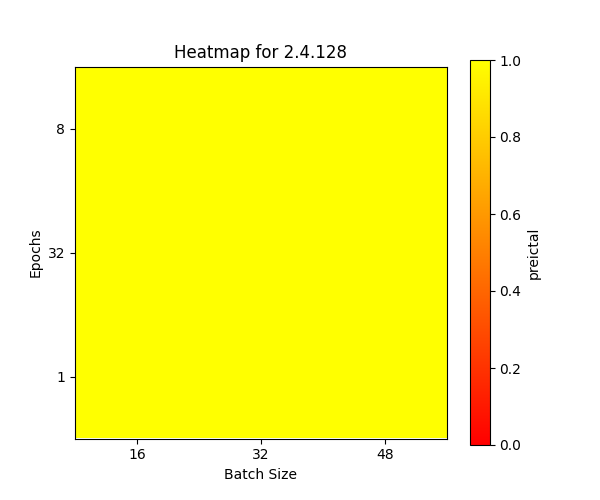
\includegraphics[width=\textwidth]{heatmap_recall_preictal_2.4.128}
\centering
\caption{Heatmap of recall for preictal class during testing for models with architecture 2.4.128.}
\label{fig:time-metrics}
\end{figure}

\begin{figure}[H]
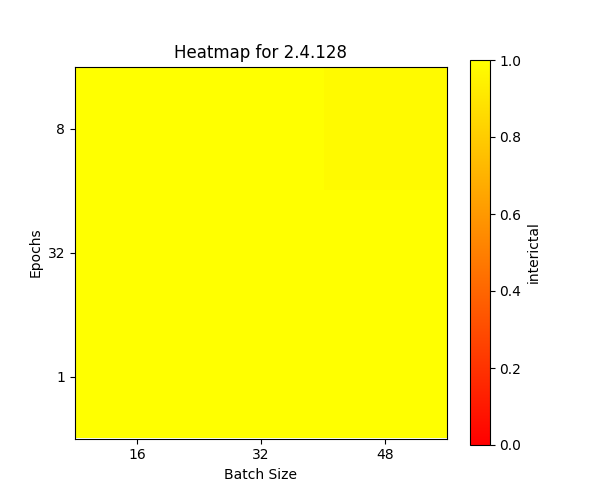
\includegraphics[width=\textwidth]{heatmap_recall_interictal_2.4.128}
\centering
\caption{Heatmap of recall for interictal class during testing for models with architecture 2.4.128.}
\label{fig:time-metrics}
\end{figure}

\begin{figure}[H]
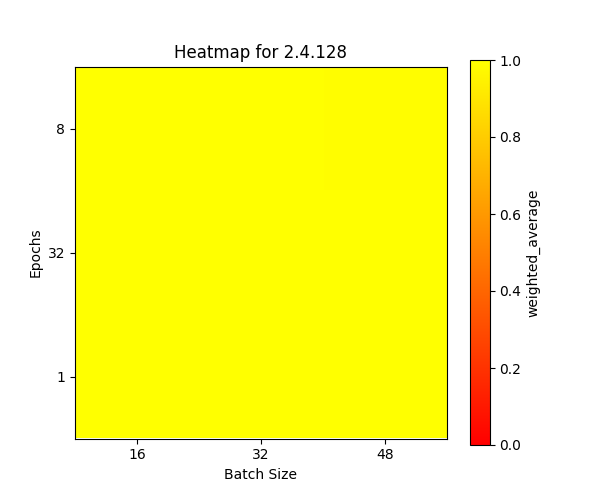
\includegraphics[width=\textwidth]{heatmap_recall_weighted_average_2.4.128}
\centering
\caption{Heatmap of recall (weighted average) during testing for models with architecture 2.4.128.}
\label{fig:time-metrics}
\end{figure}

\begin{figure}[H]
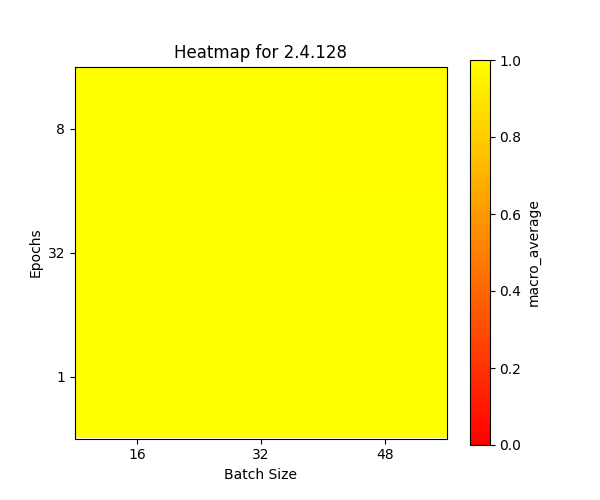
\includegraphics[width=\textwidth]{heatmap_recall_macro_average_2.4.128}
\centering
\caption{Heatmap of recall (macro average) during testing for models with architecture 2.4.128.}
\label{fig:time-metrics}
\end{figure}


\subsubsection{Testing F1}


\begin{figure}[H]
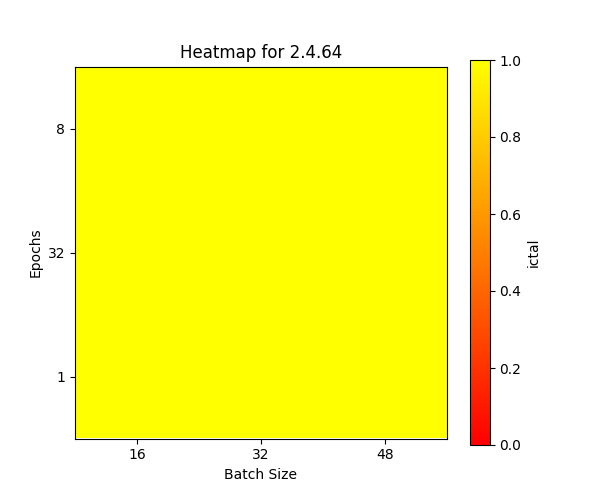
\includegraphics[width=\textwidth]{heatmap_f1_ictal_2.4.64}
\centering
\caption{Heatmap of F1 for ictal class during testing for models with architecture 2.4.64.}
\label{fig:time-metrics}
\end{figure}

\begin{figure}[H]
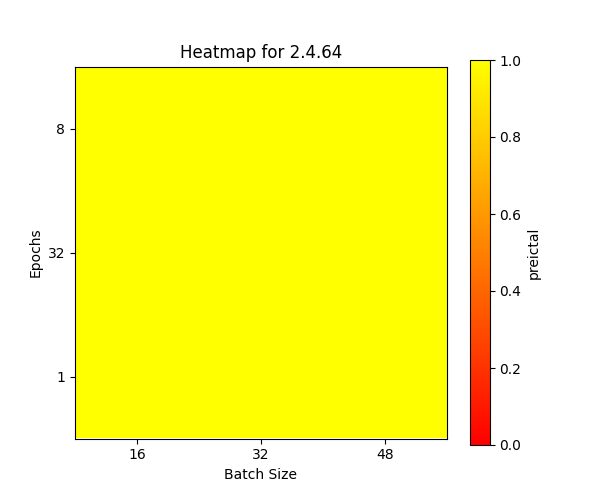
\includegraphics[width=\textwidth]{heatmap_f1_preictal_2.4.64}
\centering
\caption{Heatmap of F1 for preictal class during testing for models with architecture 2.4.64.}
\label{fig:time-metrics}
\end{figure}

\begin{figure}[H]
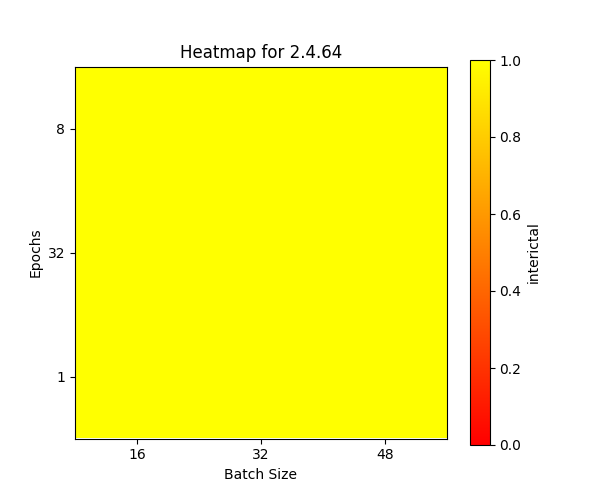
\includegraphics[width=\textwidth]{heatmap_f1_interictal_2.4.64}
\centering
\caption{Heatmap of F1 for interictal class during testing for models with architecture 2.4.64.}
\label{fig:time-metrics}
\end{figure}

\begin{figure}[H]
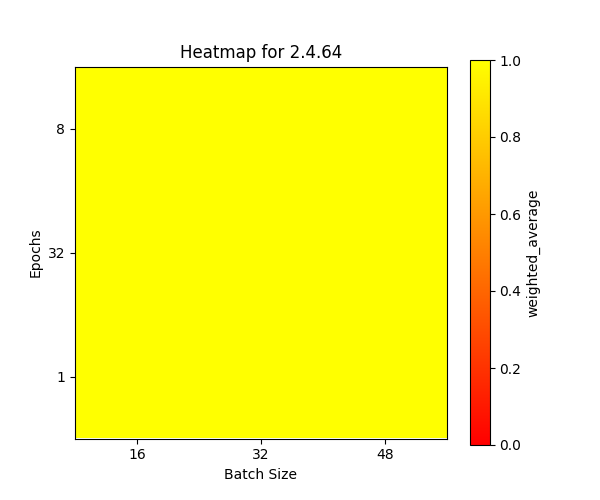
\includegraphics[width=\textwidth]{heatmap_f1_weighted_average_2.4.64}
\centering
\caption{Heatmap of F1 (weighted average) during testing for models with architecture 2.4.64.}
\label{fig:time-metrics}
\end{figure}

\begin{figure}[H]
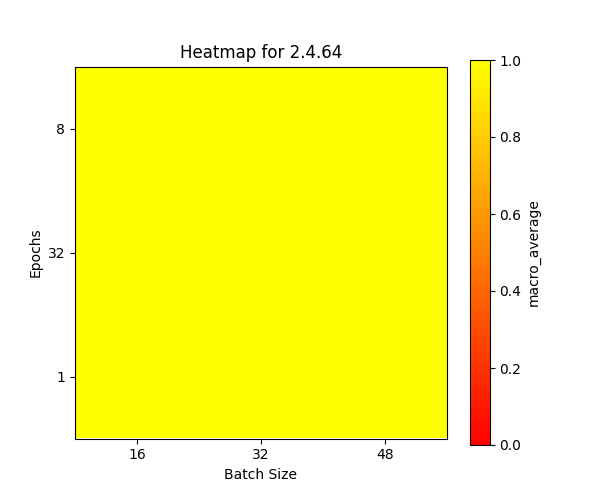
\includegraphics[width=\textwidth]{heatmap_f1_macro_average_2.4.64}
\centering
\caption{Heatmap of F1 (macro average) during testing for models with architecture 2.4.64.}
\label{fig:time-metrics}
\end{figure}


\begin{figure}[H]
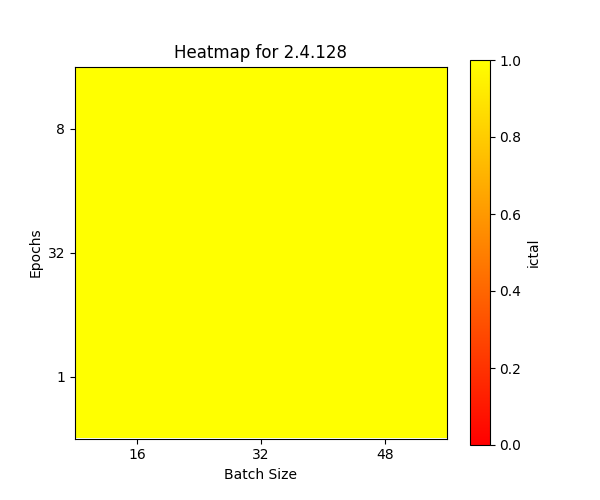
\includegraphics[width=\textwidth]{heatmap_f1_ictal_2.4.128}
\centering
\caption{Heatmap of F1 for ictal class during testing for models with architecture 2.4.128.}
\label{fig:time-metrics}
\end{figure}

\begin{figure}[H]
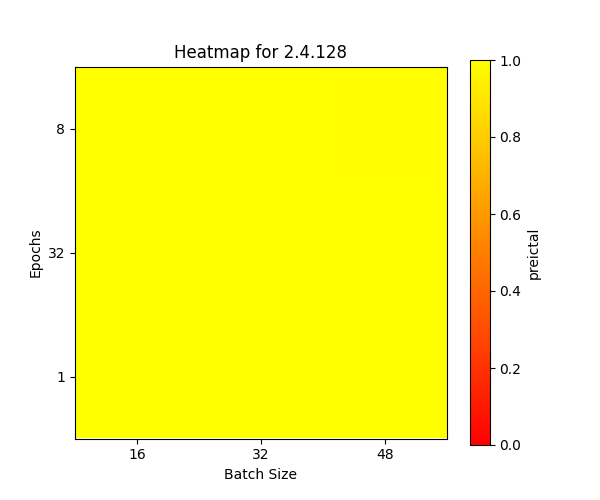
\includegraphics[width=\textwidth]{heatmap_f1_preictal_2.4.128}
\centering
\caption{Heatmap of F1 for preictal class during testing for models with architecture 2.4.128.}
\label{fig:time-metrics}
\end{figure}

\begin{figure}[H]
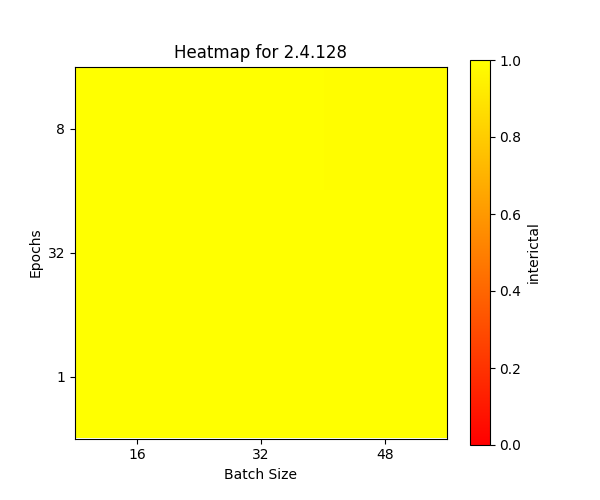
\includegraphics[width=\textwidth]{heatmap_f1_interictal_2.4.128}
\centering
\caption{Heatmap of F1 for interictal class during testing for models with architecture 2.4.128.}
\label{fig:time-metrics}
\end{figure}

\begin{figure}[H]
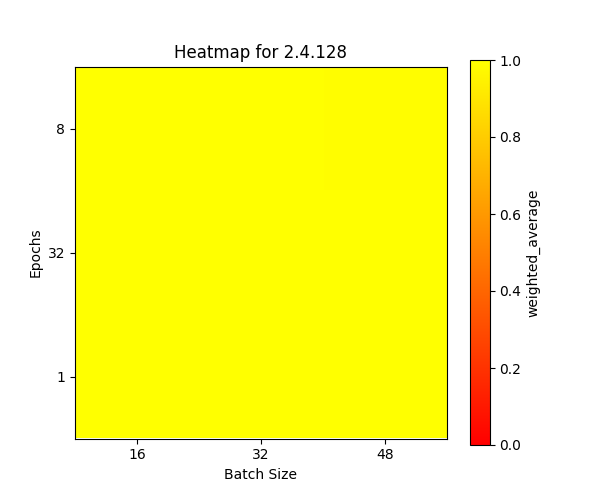
\includegraphics[width=\textwidth]{heatmap_f1_weighted_average_2.4.128}
\centering
\caption{Heatmap of F1 (weighted average) during testing for models with architecture 2.4.128.}
\label{fig:time-metrics}
\end{figure}

\begin{figure}[H]
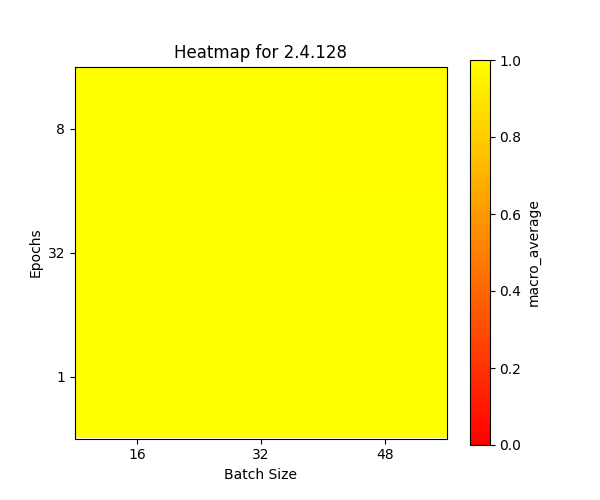
\includegraphics[width=\textwidth]{heatmap_f1_macro_average_2.4.128}
\centering
\caption{Heatmap of F1 (macro average) during testing for models with architecture 2.4.128.}
\label{fig:time-metrics}
\end{figure}



\subsubsection{Testing Precision}




\begin{figure}[H]
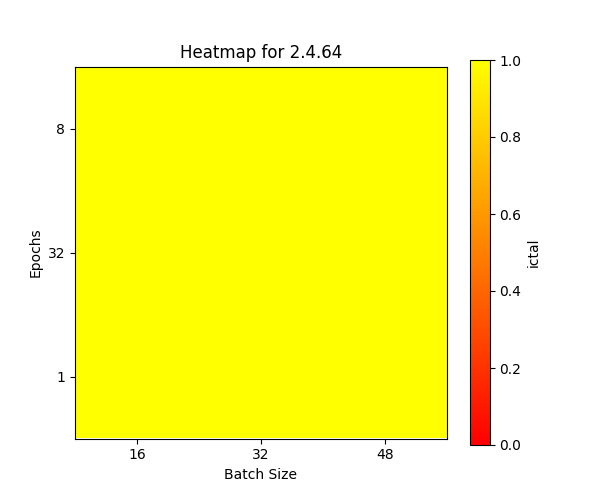
\includegraphics[width=\textwidth]{heatmap_precision_ictal_2.4.64}
\centering
\caption{Heatmap of precision for ictal class during testing for models with architecture 2.4.64.}
\label{fig:time-metrics}
\end{figure}

\begin{figure}[H]
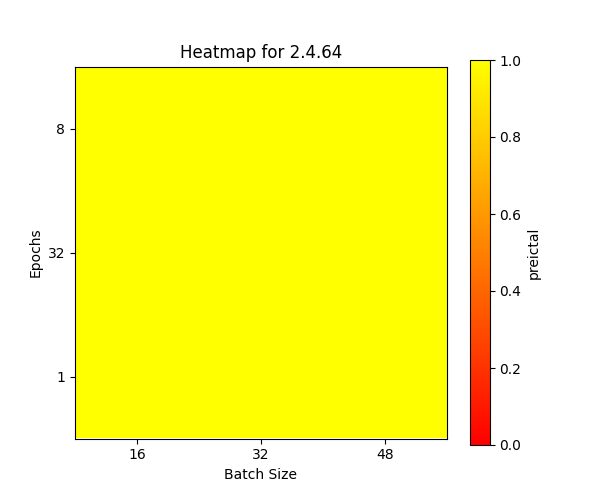
\includegraphics[width=\textwidth]{heatmap_precision_preictal_2.4.64}
\centering
\caption{Heatmap of precision for preictal class during testing for models with architecture 2.4.64.}
\label{fig:time-metrics}
\end{figure}

\begin{figure}[H]
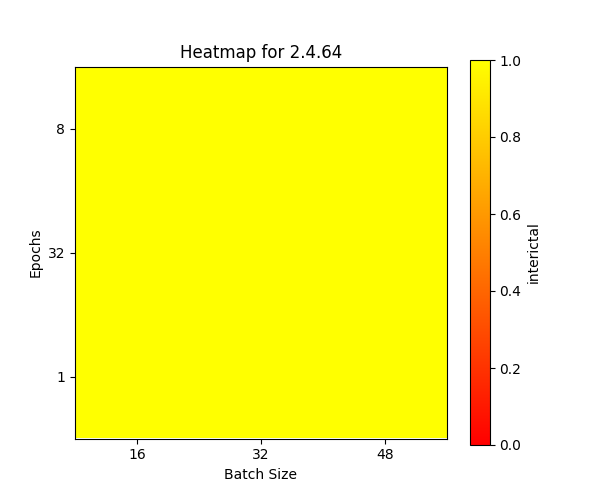
\includegraphics[width=\textwidth]{heatmap_precision_interictal_2.4.64}
\centering
\caption{Heatmap of recall for interictal class during testing for models with architecture 2.4.64.}
\label{fig:time-metrics}
\end{figure}

\begin{figure}[H]
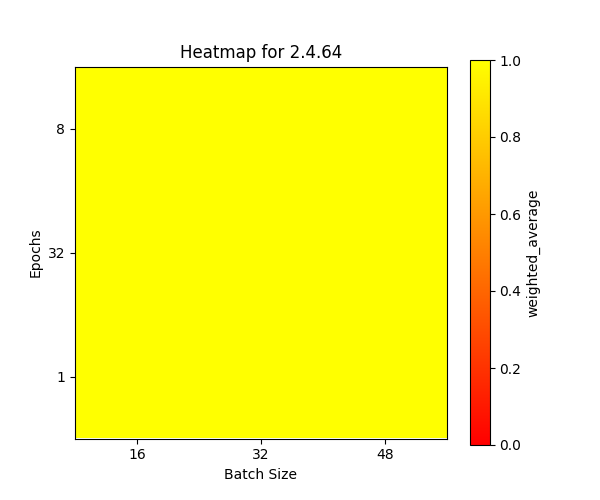
\includegraphics[width=\textwidth]{heatmap_precision_weighted_average_2.4.64}
\centering
\caption{Heatmap of precision (weighted average) during testing for models with architecture 2.4.64.}
\label{fig:time-metrics}
\end{figure}

\begin{figure}[H]
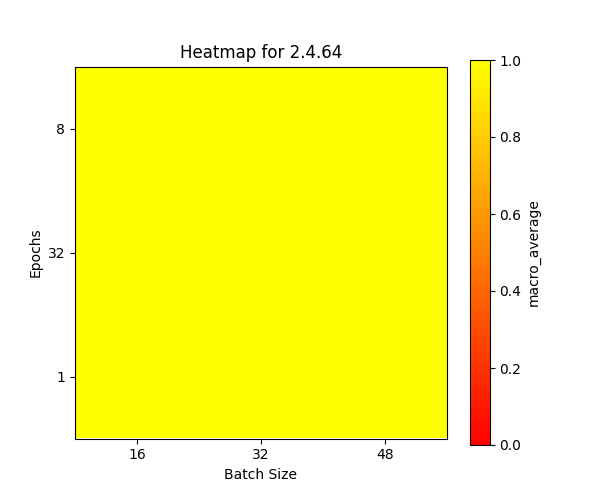
\includegraphics[width=\textwidth]{heatmap_precision_macro_average_2.4.64}
\centering
\caption{Heatmap of precision (macro average) during testing for models with architecture 2.4.64.}
\label{fig:time-metrics}
\end{figure}


\begin{figure}[H]
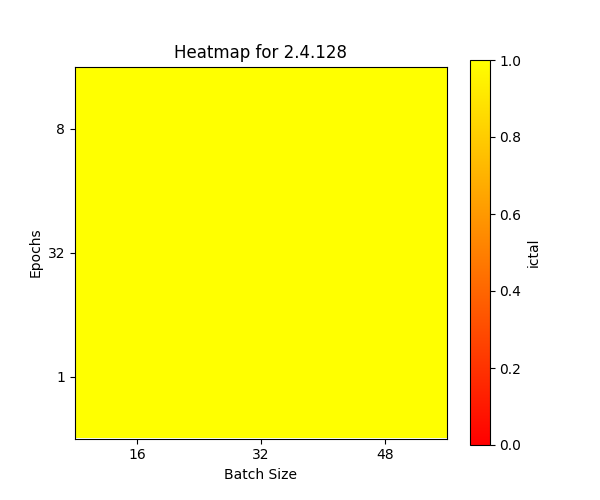
\includegraphics[width=\textwidth]{heatmap_precision_ictal_2.4.128}
\centering
\caption{Heatmap of precision for ictal class during testing for models with architecture 2.4.128.}
\label{fig:time-metrics}
\end{figure}

\begin{figure}[H]
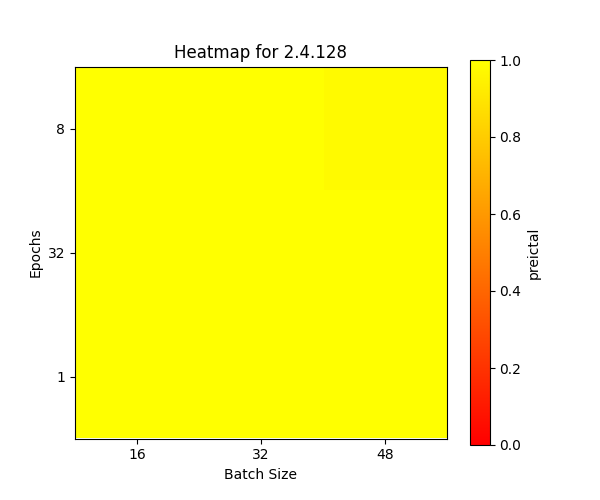
\includegraphics[width=\textwidth]{heatmap_precision_preictal_2.4.128}
\centering
\caption{Heatmap of precision for preictal class during testing for models with architecture 2.4.128.}
\label{fig:time-metrics}
\end{figure}

\begin{figure}[H]
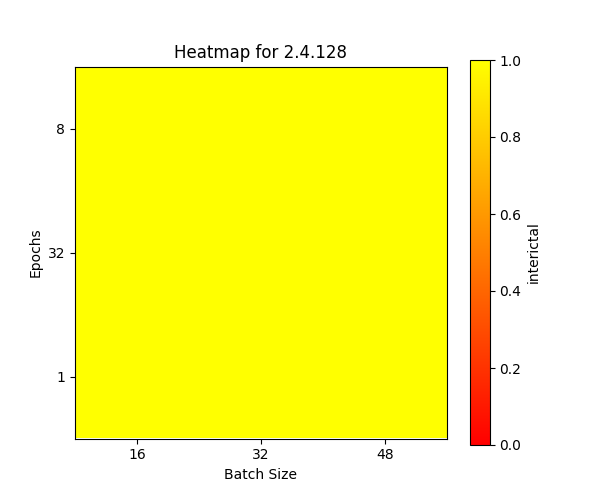
\includegraphics[width=\textwidth]{heatmap_precision_interictal_2.4.128}
\centering
\caption{Heatmap of precision for interictal class during testing for models with architecture 2.4.128.}
\label{fig:time-metrics}
\end{figure}

\begin{figure}[H]
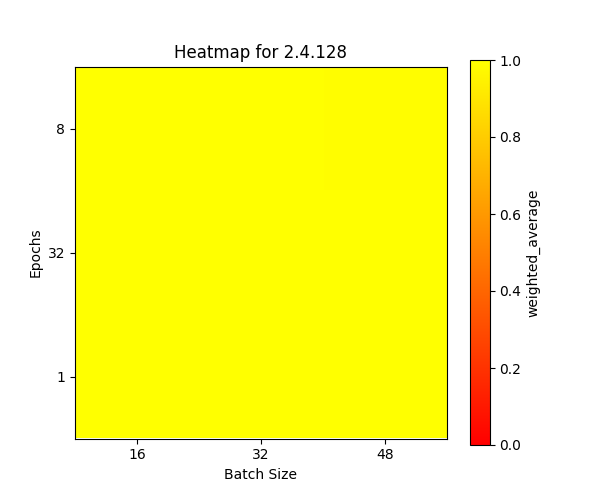
\includegraphics[width=\textwidth]{heatmap_precision_weighted_average_2.4.128}
\centering
\caption{Heatmap of precision (weighted average) during testing for models with architecture 2.4.128.}
\label{fig:time-metrics}
\end{figure}

\begin{figure}[H]
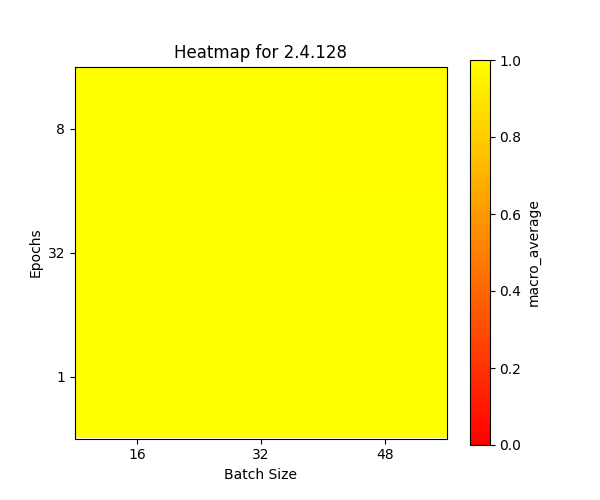
\includegraphics[width=\textwidth]{heatmap_precision_macro_average_2.4.128}
\centering
\caption{Heatmap of precision (macro average) during testing for models with architecture 2.4.128.}
\label{fig:time-metrics}
\end{figure}





\section{Misc.}

\begin{lstlisting}[style=logstyle, caption={Example Summary file from the \acrshort{chb} \acrshort{eeg} dataset.}, label={lst:summary-file}]
File Name: chb06_03.edf
File Start Time: 03:09:42
File End Time: 7:09:42
Number of Seizures in File: 0

File Name: chb06_04.edf
File Start Time: 07:09:51
File End Time: 10:50:52
Number of Seizures in File: 2
Seizure 1 Start Time: 327 seconds
Seizure 1 End Time: 347 seconds
Seizure 2 Start Time: 6211 seconds
Seizure 2 End Time: 6231 seconds

File Name: chb06_05.edf
File Start Time: 10:51:20
File End Time: 14:51:20
Number of Seizures in File: 0

File Name: chb06_06.edf
File Start Time: 14:51:23
File End Time: 18:51:23
Number of Seizures in File: 0

File Name: chb06_07.edf
File Start Time: 18:51:31
File End Time: 22:51:31
Number of Seizures in File: 0

File Name: chb06_08.edf
File Start Time: 22:51:39
File End Time: 26:51:39
Number of Seizures in File: 0

File Name: chb06_09.edf
File Start Time: 02:51:47
File End Time: 6:51:47
Number of Seizures in File: 1
Seizure 1 Start Time: 12500 seconds
Seizure 1 End Time: 12516 seconds

File Name: chb06_10.edf
File Start Time: 06:51:54
File End Time: 10:51:54
Number of Seizures in File: 1
Seizure 1 Start Time: 10833 seconds
Seizure 1 End Time: 10845 seconds

File Name: chb06_12.edf
File Start Time: 14:52:10
File End Time: 18:52:10
Number of Seizures in File: 0

File Name: chb06_13.edf
File Start Time: 18:52:20
File End Time: 22:52:20
Number of Seizures in File: 1
Seizure 1 Start Time: 506 seconds
Seizure 1 End Time: 519 seconds

File Name: chb06_14.edf
File Start Time: 22:52:35
File End Time: 26:52:35
Number of Seizures in File: 0

File Name: chb06_15.edf
File Start Time: 02:52:43
File End Time: 6:52:43
Number of Seizures in File: 0

File Name: chb06_16.edf
File Start Time: 06:52:51
File End Time: 7:43:21
Number of Seizures in File: 0

File Name: chb06_17.edf
File Start Time: 07:45:51
File End Time: 11:45:51
Number of Seizures in File: 0

File Name: chb06_18.edf
File Start Time: 11:45:55
File End Time: 13:58:03
Number of Seizures in File: 1
Seizure 1 Start Time: 7799 seconds
Seizure 1 End Time: 7811 seconds

File Name: chb06_24.edf
File Start Time: 08:23:24
File End Time: 12:23:24
Number of Seizures in File: 1
Seizure 1 Start Time: 9387 seconds
Seizure 1 End Time: 9403 seconds
\end{lstlisting}




\begin{figure}[H]
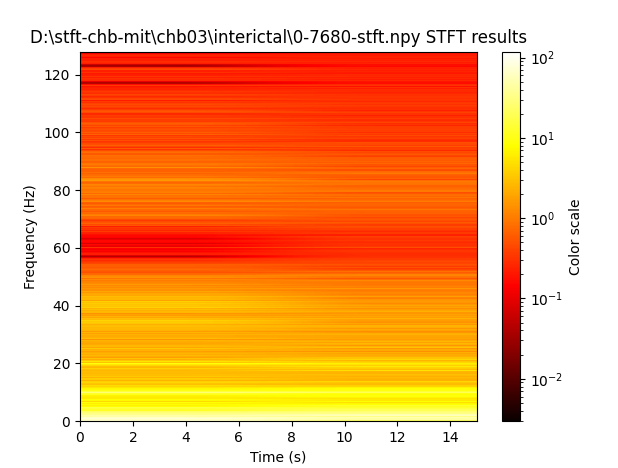
\includegraphics[width=\textwidth]{stft2}
\centering
\caption{An STFT window with high time resolution.}
\label{fig:stft2}
\end{figure}


\begin{lstlisting}[style=logstyle, caption={List of failed trained models. See \ref{issues}}, label={lst:model-list}]
/data/results-archive/2.4.128/16.1.keras
/data/results-archive/2.4.128/16.32.keras
/data/results-archive/2.4.128/16.8.keras
/data/results-archive/2.4.128/32.1.keras
/data/results-archive/2.4.128/32.32.keras
/data/results-archive/2.4.128/32.8.keras
/data/results-archive/2.4.128/48.1.keras
/data/results-archive/2.4.128/48.8.keras
/data/results-archive/2.4.256/16.1.keras
/data/results-archive/2.4.256/16.32.keras
/data/results-archive/2.4.256/16.8.keras
/data/results-archive/2.4.256/32.1.keras
/data/results-archive/2.4.256/32.32.keras
/data/results-archive/2.4.256/32.8.keras
/data/results-archive/2.4.256/48.1.keras
/data/results-archive/2.4.256/48.32.keras
/data/results-archive/2.4.256/48.8.keras
/data/results-archive/2.4.64/16.1.keras
/data/results-archive/2.4.64/16.32.keras
/data/results-archive/2.4.64/16.8.keras
/data/results-archive/2.4.64/32.1.keras
/data/results-archive/2.4.64/32.32.keras
/data/results-archive/2.4.64/32.8.keras
/data/results-archive/2.4.64/48.1.keras
/data/results-archive/2.4.64/48.32.keras
/data/results-archive/2.4.64/48.8.keras
/data/results-archive/2.8.64/16.1.keras
/data/results-archive/2.8.64/16.32.keras
/data/results-archive/2.8.64/16.8.keras
/data/results-archive/2.8.64/32.1.keras
/data/results-archive/2.8.64/32.32.keras
/data/results-archive/2.8.64/32.8.keras
/data/results-archive/2.8.64/48.1.keras
/data/results-archive/2.8.64/48.8.keras
/data/results-archive/48.32.keras
/data/results-archive/ictal-only-prediction/2.12.128/16.1.keras
/data/results-archive/ictal-only-prediction/2.12.128/16.8.keras
/data/results-archive/ictal-only-prediction/2.12.128/32.1.keras
/data/results-archive/ictal-only-prediction/2.12.128/32.8.keras
/data/results-archive/ictal-only-prediction/2.12.256/16.1.keras
/data/results-archive/ictal-only-prediction/2.12.256/16.8.keras
/data/results-archive/ictal-only-prediction/2.12.256/32.1.keras
/data/results-archive/ictal-only-prediction/2.12.256/32.8.keras
/data/results-archive/ictal-only-prediction/2.12.64/16.1.keras
/data/results-archive/ictal-only-prediction/2.12.64/16.8.keras
/data/results-archive/ictal-only-prediction/2.12.64/32.1.keras
/data/results-archive/ictal-only-prediction/2.12.64/32.8.keras
/data/results-archive/ictal-only-prediction/2.4.128/16.1.keras
/data/results-archive/ictal-only-prediction/2.4.128/16.8.keras
/data/results-archive/ictal-only-prediction/2.4.128/32.1.keras
/data/results-archive/ictal-only-prediction/2.4.128/32.8.keras
/data/results-archive/ictal-only-prediction/2.4.256/16.1.keras
/data/results-archive/ictal-only-prediction/2.4.256/16.8.keras
/data/results-archive/ictal-only-prediction/2.4.256/32.1.keras
/data/results-archive/ictal-only-prediction/2.4.256/32.8.keras
/data/results-archive/ictal-only-prediction/2.4.64/16.1.keras
/data/results-archive/ictal-only-prediction/2.4.64/16.8.keras
/data/results-archive/ictal-only-prediction/2.4.64/32.1.keras
/data/results-archive/ictal-only-prediction/2.4.64/32.8.keras
/data/results-archive/ictal-only-prediction/2.8.128/16.1.keras
/data/results-archive/ictal-only-prediction/2.8.128/16.8.keras
/data/results-archive/ictal-only-prediction/2.8.128/32.1.keras
/data/results-archive/ictal-only-prediction/2.8.128/32.8.keras
/data/results-archive/ictal-only-prediction/2.8.256/16.1.keras
/data/results-archive/ictal-only-prediction/2.8.256/16.8.keras
/data/results-archive/ictal-only-prediction/2.8.256/32.1.keras
/data/results-archive/ictal-only-prediction/2.8.256/32.8.keras
/data/results-archive/ictal-only-prediction/2.8.64/16.1.keras
/data/results-archive/ictal-only-prediction/2.8.64/16.8.keras
/data/results-archive/ictal-only-prediction/2.8.64/32.1.keras
/data/results-archive/ictal-only-prediction/2.8.64/32.8.keras
/data/results-archive/imbalanced_training/2.4.64/16.1.keras
/data/results-archive/imbalanced_training/2.4.64/16.8.keras
/data/results-archive/imbalanced_training/2.4.64/32.1.keras
/data/results-archive/imbalanced_training/2.4.64/32.8.keras
/data/results-archive/imbalanced_training_2/2.12.128/16.1.keras
/data/results-archive/imbalanced_training_2/2.12.128/16.8.keras
/data/results-archive/imbalanced_training_2/2.12.128/32.1.keras
/data/results-archive/imbalanced_training_2/2.12.128/32.8.keras
/data/results-archive/imbalanced_training_2/2.12.256/16.1.keras
/data/results-archive/imbalanced_training_2/2.12.256/16.8.keras
/data/results-archive/imbalanced_training_2/2.12.256/32.1.keras
/data/results-archive/imbalanced_training_2/2.12.256/32.8.keras
/data/results-archive/imbalanced_training_2/2.12.64/16.1.keras
/data/results-archive/imbalanced_training_2/2.12.64/16.8.keras
/data/results-archive/imbalanced_training_2/2.12.64/32.1.keras
/data/results-archive/imbalanced_training_2/2.12.64/32.8.keras
/data/results-archive/imbalanced_training_2/2.4.128/16.1.keras
/data/results-archive/imbalanced_training_2/2.4.128/16.8.keras
/data/results-archive/imbalanced_training_2/2.4.128/32.1.keras
/data/results-archive/imbalanced_training_2/2.4.128/32.8.keras
/data/results-archive/imbalanced_training_2/2.4.256/16.1.keras
/data/results-archive/imbalanced_training_2/2.4.256/16.8.keras
/data/results-archive/imbalanced_training_2/2.4.256/32.1.keras
/data/results-archive/imbalanced_training_2/2.4.256/32.8.keras
/data/results-archive/imbalanced_training_2/2.4.64/16.1.keras
/data/results-archive/imbalanced_training_2/2.4.64/16.8.keras
/data/results-archive/imbalanced_training_2/2.4.64/32.1.keras
/data/results-archive/imbalanced_training_2/2.4.64/32.8.keras
/data/results-archive/imbalanced_training_2/2.8.128/16.1.keras
/data/results-archive/imbalanced_training_2/2.8.128/16.8.keras
/data/results-archive/imbalanced_training_2/2.8.128/32.1.keras
/data/results-archive/imbalanced_training_2/2.8.128/32.8.keras
/data/results-archive/imbalanced_training_2/2.8.256/16.1.keras
/data/results-archive/imbalanced_training_2/2.8.256/16.8.keras
/data/results-archive/imbalanced_training_2/2.8.256/32.1.keras
/data/results-archive/imbalanced_training_2/2.8.256/32.8.keras
/data/results-archive/imbalanced_training_2/2.8.64/16.1.keras
/data/results-archive/imbalanced_training_2/2.8.64/16.8.keras
/data/results-archive/imbalanced_training_2/2.8.64/32.1.keras
/data/results-archive/imbalanced_training_2/2.8.64/32.8.keras
/data/results-archive/results/2.4.64/16.1.keras
/data/results-archive/results/2.4.64/16.8.keras
/data/results-archive/results/2.4.64/32.1.keras
/data/results-archive/results - Copy/2.4.64/32.1.keras
/data/results-archive/results - Copy/4.4.64/32.4.keras
/data/results-archive/training_data_broken/2.12.128/16.1.keras
/data/results-archive/training_data_broken/2.12.128/16.32.keras
/data/results-archive/training_data_broken/2.12.128/16.8.keras
/data/results-archive/training_data_broken/2.12.128/32.1.keras
/data/results-archive/training_data_broken/2.12.128/32.32.keras
/data/results-archive/training_data_broken/2.12.128/32.8.keras
/data/results-archive/training_data_broken/2.12.128/48.1.keras
/data/results-archive/training_data_broken/2.12.128/48.32.keras
/data/results-archive/training_data_broken/2.12.128/48.8.keras
/data/results-archive/training_data_broken/2.12.256/16.1.keras
/data/results-archive/training_data_broken/2.12.256/16.32.keras
/data/results-archive/training_data_broken/2.12.256/16.8.keras
/data/results-archive/training_data_broken/2.12.256/32.1.keras
/data/results-archive/training_data_broken/2.12.256/32.32.keras
/data/results-archive/training_data_broken/2.12.256/32.8.keras
/data/results-archive/training_data_broken/2.12.256/48.1.keras
/data/results-archive/training_data_broken/2.12.256/48.32.keras
/data/results-archive/training_data_broken/2.12.256/48.8.keras
/data/results-archive/training_data_broken/2.12.64/16.1.keras
/data/results-archive/training_data_broken/2.12.64/16.32.keras
/data/results-archive/training_data_broken/2.12.64/16.8.keras
/data/results-archive/training_data_broken/2.12.64/32.1.keras
/data/results-archive/training_data_broken/2.12.64/32.32.keras
/data/results-archive/training_data_broken/2.12.64/32.8.keras
/data/results-archive/training_data_broken/2.12.64/48.1.keras
/data/results-archive/training_data_broken/2.12.64/48.32.keras
/data/results-archive/training_data_broken/2.12.64/48.8.keras
/data/results-archive/training_data_broken/2.4.256/16.1.keras
/data/results-archive/training_data_broken/2.4.256/16.32.keras
/data/results-archive/training_data_broken/2.4.256/16.8.keras
/data/results-archive/training_data_broken/2.4.256/32.1.keras
/data/results-archive/training_data_broken/2.4.256/32.32.keras
/data/results-archive/training_data_broken/2.4.256/32.8.keras
/data/results-archive/training_data_broken/2.4.256/48.1.keras
/data/results-archive/training_data_broken/2.4.256/48.32.keras
/data/results-archive/training_data_broken/2.4.256/48.8.keras
/data/results-archive/training_data_broken/2.8.128/16.1.keras
/data/results-archive/training_data_broken/2.8.128/16.32.keras
/data/results-archive/training_data_broken/2.8.128/16.8.keras
/data/results-archive/training_data_broken/2.8.128/32.1.keras
/data/results-archive/training_data_broken/2.8.128/32.32.keras
/data/results-archive/training_data_broken/2.8.128/32.8.keras
/data/results-archive/training_data_broken/2.8.128/48.1.keras
/data/results-archive/training_data_broken/2.8.128/48.32.keras
/data/results-archive/training_data_broken/2.8.128/48.8.keras
/data/results-archive/training_data_broken/2.8.256/16.1.keras
/data/results-archive/training_data_broken/2.8.256/16.32.keras
/data/results-archive/training_data_broken/2.8.256/16.8.keras
/data/results-archive/training_data_broken/2.8.256/32.1.keras
/data/results-archive/training_data_broken/2.8.256/32.32.keras
/data/results-archive/training_data_broken/2.8.256/32.8.keras
/data/results-archive/training_data_broken/2.8.256/48.1.keras
/data/results-archive/training_data_broken/2.8.256/48.32.keras
/data/results-archive/training_data_broken/2.8.256/48.8.keras
/data/results-archive/training_data_broken/2.8.64/16.1.keras
/data/results-archive/training_data_broken/2.8.64/16.32.keras
/data/results-archive/training_data_broken/2.8.64/16.8.keras
/data/results-archive/training_data_broken/2.8.64/32.1.keras
/data/results-archive/training_data_broken/2.8.64/32.32.keras
/data/results-archive/training_data_broken/2.8.64/32.8.keras
/data/results-archive/training_data_broken/2.8.64/48.1.keras
/data/results-archive/training_data_broken/2.8.64/48.32.keras
/data/results-archive/training_data_broken/2.8.64/48.8.keras
/data/results-archive/training_data_broken/3.12.128/16.1.keras
/data/results-archive/training_data_broken/3.12.128/16.32.keras
/data/results-archive/training_data_broken/3.12.128/16.8.keras
/data/results-archive/training_data_broken/3.12.128/32.1.keras
/data/results-archive/training_data_broken/3.12.128/32.32.keras
/data/results-archive/training_data_broken/3.12.128/32.8.keras
/data/results-archive/training_data_broken/3.12.128/48.1.keras
/data/results-archive/training_data_broken/3.12.128/48.32.keras
/data/results-archive/training_data_broken/3.12.128/48.8.keras
/data/results-archive/training_data_broken/3.12.256/16.1.keras
/data/results-archive/training_data_broken/3.12.256/16.32.keras
/data/results-archive/training_data_broken/3.12.256/16.8.keras
/data/results-archive/training_data_broken/3.12.256/32.1.keras
/data/results-archive/training_data_broken/3.12.256/32.32.keras
/data/results-archive/training_data_broken/3.12.256/32.8.keras
/data/results-archive/training_data_broken/3.12.256/48.1.keras
/data/results-archive/training_data_broken/3.12.256/48.32.keras
/data/results-archive/training_data_broken/3.12.256/48.8.keras
/data/results-archive/training_data_broken/3.12.64/16.1.keras
/data/results-archive/training_data_broken/3.12.64/16.32.keras
/data/results-archive/training_data_broken/3.12.64/16.8.keras
/data/results-archive/training_data_broken/3.12.64/32.1.keras
/data/results-archive/training_data_broken/3.12.64/32.32.keras
/data/results-archive/training_data_broken/3.12.64/32.8.keras
/data/results-archive/training_data_broken/3.12.64/48.1.keras
/data/results-archive/training_data_broken/3.12.64/48.32.keras
/data/results-archive/training_data_broken/3.12.64/48.8.keras
/data/results-archive/training_data_broken/3.4.128/16.1.keras
/data/results-archive/training_data_broken/3.4.128/16.32.keras
/data/results-archive/training_data_broken/3.4.128/16.8.keras
/data/results-archive/training_data_broken/3.4.128/32.1.keras
/data/results-archive/training_data_broken/3.4.128/32.32.keras
/data/results-archive/training_data_broken/3.4.128/32.8.keras
/data/results-archive/training_data_broken/3.4.128/48.1.keras
/data/results-archive/training_data_broken/3.4.128/48.32.keras
/data/results-archive/training_data_broken/3.4.128/48.8.keras
/data/results-archive/training_data_broken/3.4.256/16.1.keras
/data/results-archive/training_data_broken/3.4.256/16.32.keras
/data/results-archive/training_data_broken/3.4.256/16.8.keras
/data/results-archive/training_data_broken/3.4.256/32.1.keras
/data/results-archive/training_data_broken/3.4.256/32.32.keras
/data/results-archive/training_data_broken/3.4.256/32.8.keras
/data/results-archive/training_data_broken/3.4.256/48.1.keras
/data/results-archive/training_data_broken/3.4.256/48.32.keras
/data/results-archive/training_data_broken/3.4.256/48.8.keras
/data/results-archive/training_data_broken/3.4.64/16.1.keras
/data/results-archive/training_data_broken/3.4.64/16.32.keras
/data/results-archive/training_data_broken/3.4.64/16.8.keras
/data/results-archive/training_data_broken/3.4.64/32.1.keras
/data/results-archive/training_data_broken/3.4.64/32.32.keras
/data/results-archive/training_data_broken/3.4.64/32.8.keras
/data/results-archive/training_data_broken/3.4.64/48.1.keras
/data/results-archive/training_data_broken/3.4.64/48.32.keras
/data/results-archive/training_data_broken/3.4.64/48.8.keras
/data/results-archive/training_data_broken/3.8.128/16.1.keras
/data/results-archive/training_data_broken/3.8.128/16.32.keras
/data/results-archive/training_data_broken/3.8.128/16.8.keras
/data/results-archive/training_data_broken/3.8.128/32.1.keras
/data/results-archive/training_data_broken/3.8.128/32.32.keras
/data/results-archive/training_data_broken/3.8.128/32.8.keras
/data/results-archive/training_data_broken/3.8.128/48.1.keras
/data/results-archive/training_data_broken/3.8.128/48.32.keras
/data/results-archive/training_data_broken/3.8.128/48.8.keras
/data/results-archive/training_data_broken/3.8.256/16.1.keras
/data/results-archive/training_data_broken/3.8.256/16.32.keras
/data/results-archive/training_data_broken/3.8.256/16.8.keras
/data/results-archive/training_data_broken/3.8.256/32.1.keras
/data/results-archive/training_data_broken/3.8.256/32.32.keras
/data/results-archive/training_data_broken/3.8.256/32.8.keras
/data/results-archive/training_data_broken/3.8.256/48.1.keras
/data/results-archive/training_data_broken/3.8.256/48.32.keras
/data/results-archive/training_data_broken/3.8.256/48.8.keras
/data/results-archive/training_data_broken/3.8.64/16.1.keras
/data/results-archive/training_data_broken/3.8.64/16.32.keras
/data/results-archive/training_data_broken/3.8.64/16.8.keras
/data/results-archive/training_data_broken/3.8.64/32.1.keras
/data/results-archive/training_data_broken/3.8.64/32.32.keras
/data/results-archive/training_data_broken/3.8.64/32.8.keras
/data/results-archive/training_data_broken/3.8.64/48.1.keras
/data/results-archive/training_data_broken/3.8.64/48.32.keras
/data/results-archive/training_data_broken/3.8.64/48.8.keras
/data/results-combined/2.4.16/16.1.keras
/data/results-combined/2.4.16/16.32.keras
/data/results-combined/2.4.16/16.8.keras
/data/results-test/2.4.128/16.1.keras
/data/results-test/2.4.128/16.32.keras
/data/results-test/2.4.128/16.8.keras
/data/results-test/2.4.128/32.1.keras
/data/results-test/2.4.128/32.32.keras
/data/results-test/2.4.128/32.8.keras
/data/results-test/2.4.128/48.1.keras
/data/results-test/2.4.128/48.8.keras
/data/results-test/2.4.64/16.1.keras
/data/results-test/2.4.64/16.32.keras
/data/results-test/2.4.64/16.8.keras
/data/results-test/2.4.64/32.1.keras
/data/results-test/2.4.64/32.32.keras
/data/results-test/2.4.64/32.8.keras
/data/results-test/2.4.64/48.1.keras
/data/results-test/2.4.64/48.32.keras
/data/results-test/2.4.64/48.8.keras
\end{lstlisting}




\section{Presentation, Poster, and Ethics Form}

\includepdf[pages=-, landscape]{presentation.pdf}
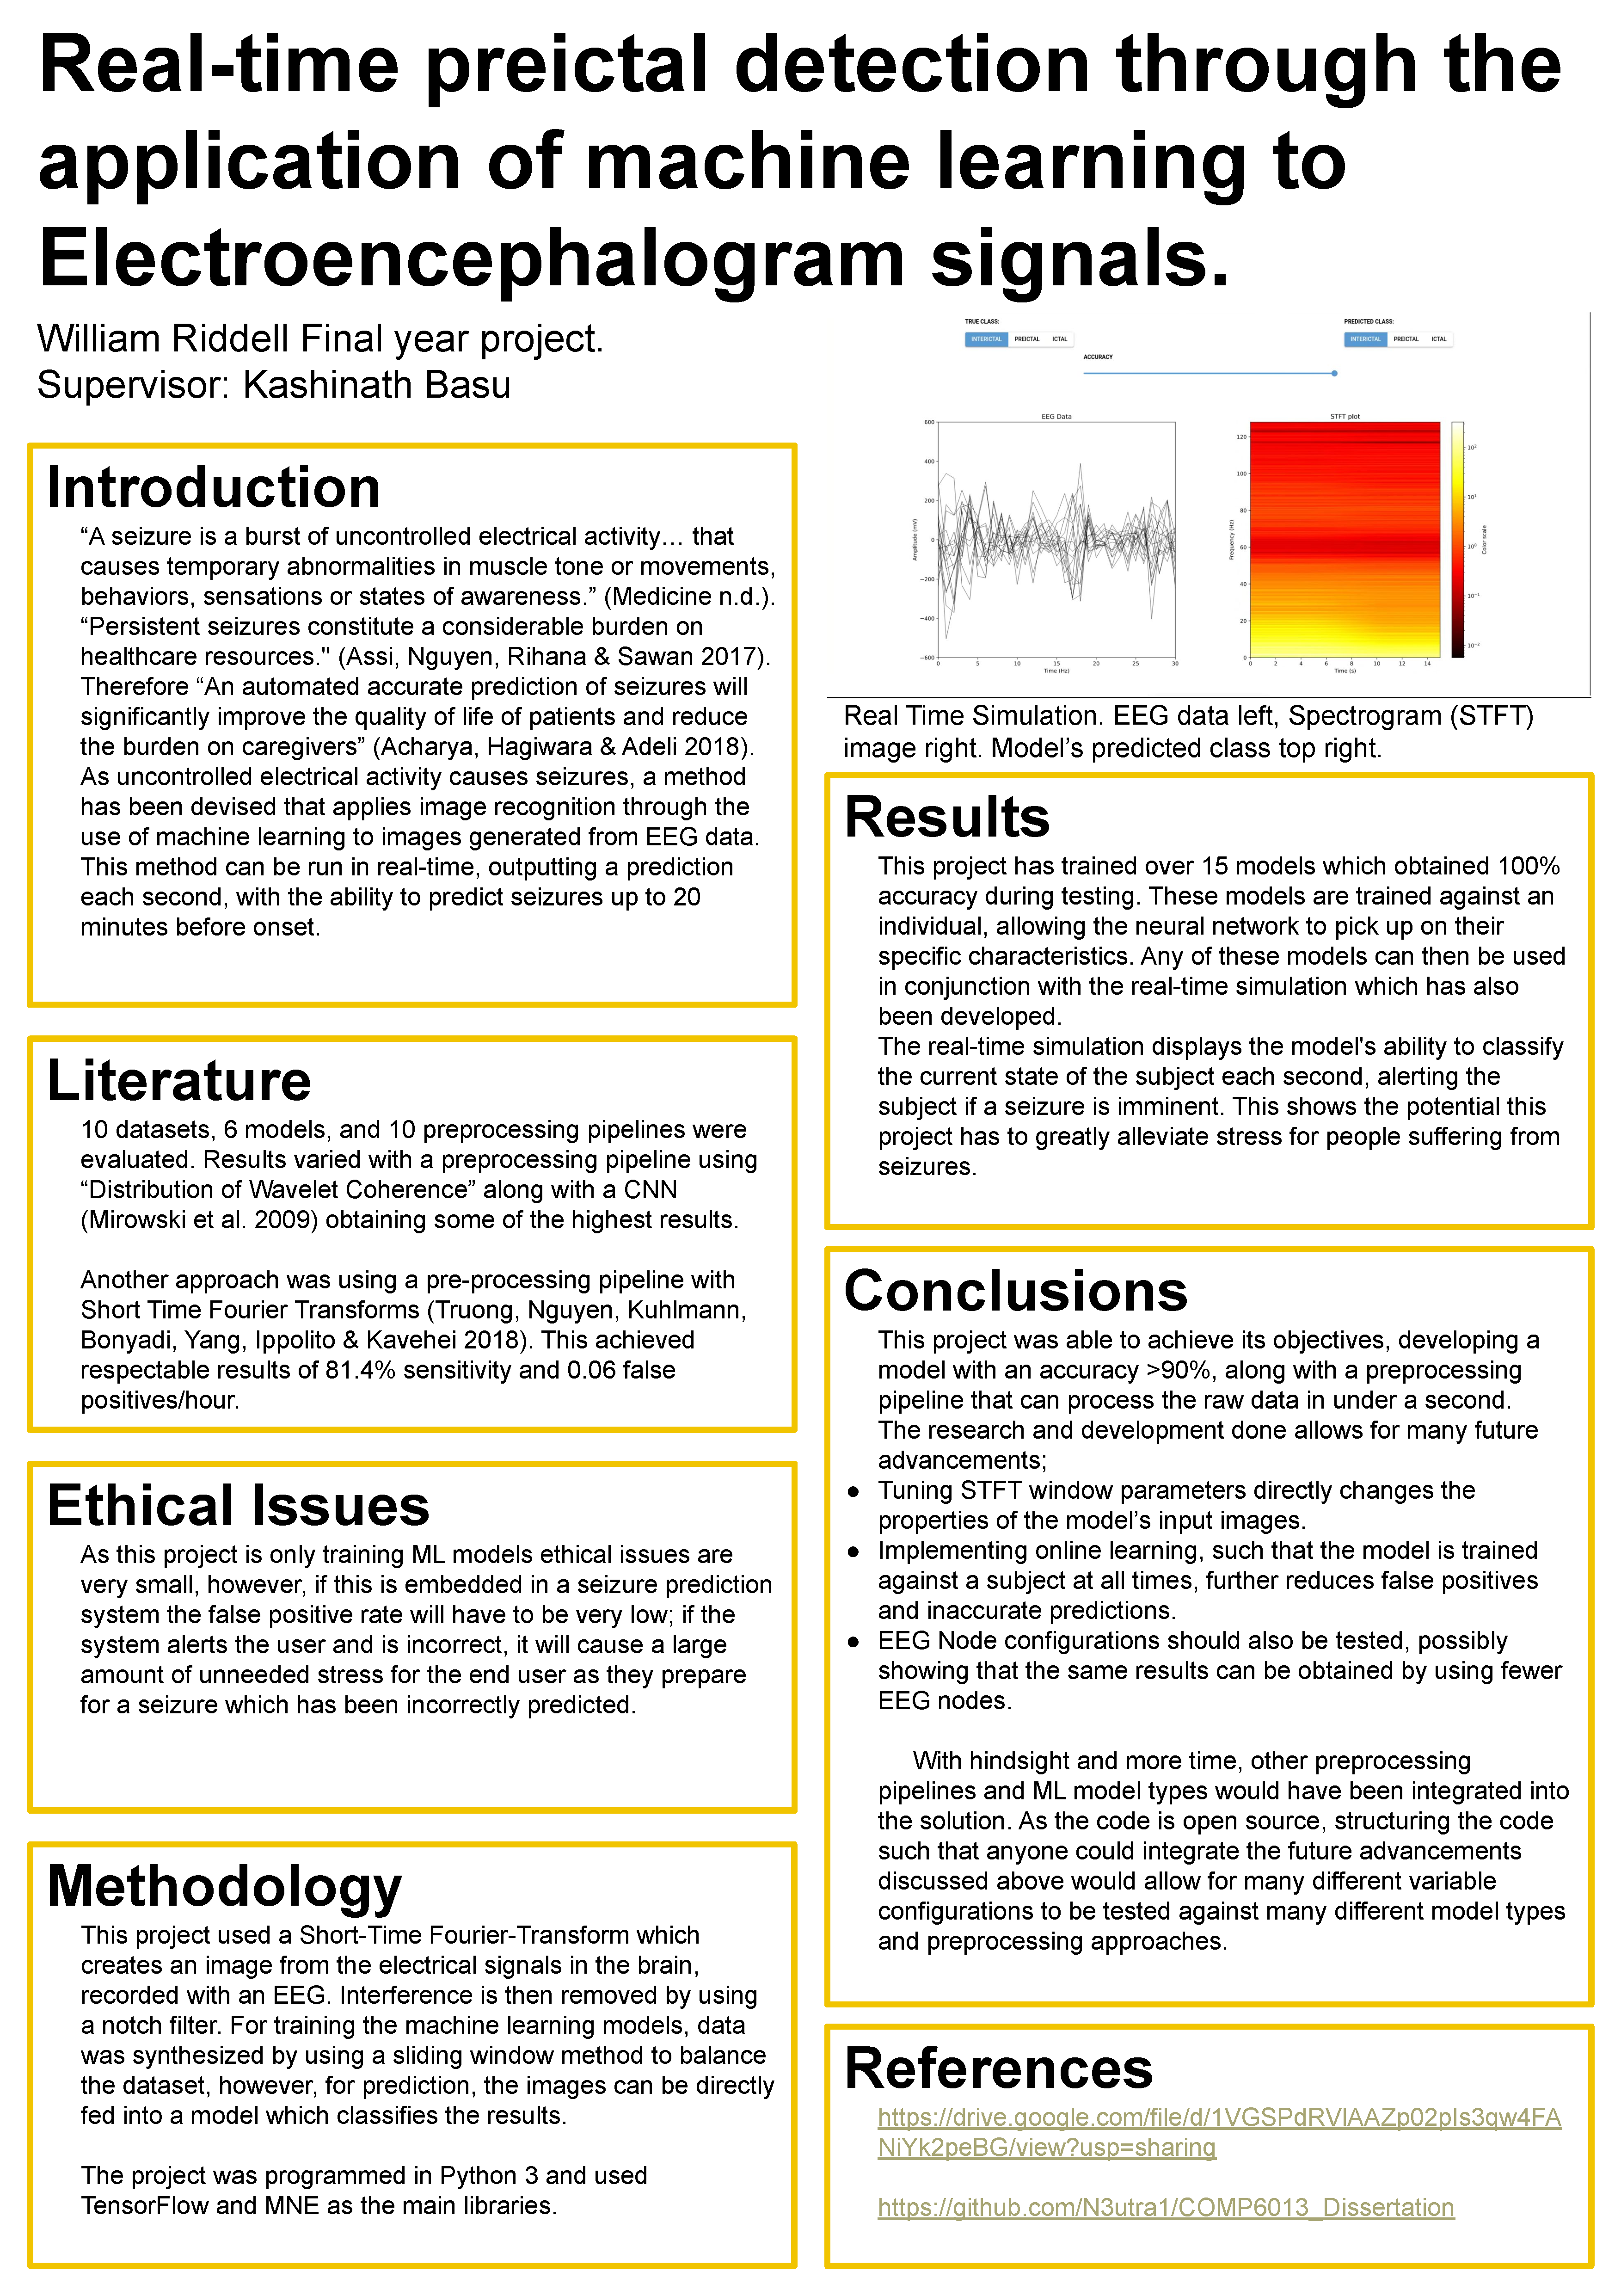
\includepdf[pages=-]{poster.pdf}

\includepdf[pages=-]{tde_e1.pdf}

\end{document}